%%% The main file. It contains definitions of basic parameters and includes all other parts.

%% Settings for single-side (simplex) printing
% Margins: left 40mm, right 25mm, top and bottom 25mm
% (but beware, LaTeX adds 1in implicitly)
\documentclass[12pt,a4paper]{report}
\setlength\textwidth{145mm}
\setlength\textheight{247mm}
\setlength\oddsidemargin{15mm}
\setlength\evensidemargin{15mm}
\setlength\topmargin{0mm}
\setlength\headsep{0mm}
\setlength\headheight{0mm}
% \openright makes the following text appear on a right-hand page
\let\openright=\clearpage

%% Settings for two-sided (duplex) printing
% \documentclass[12pt,a4paper,twoside,openright]{report}
% \setlength\textwidth{145mm}
% \setlength\textheight{247mm}
% \setlength\oddsidemargin{14.2mm}
% \setlength\evensidemargin{0mm}
% \setlength\topmargin{0mm}
% \setlength\headsep{0mm}
% \setlength\headheight{0mm}
% \let\openright=\cleardoublepage

%% Generate PDF/A-2u
\usepackage[a-2u]{pdfx}

%% Character encoding: usually latin2, cp1250 or utf8:
\usepackage[utf8]{inputenc}

%% Prefer Latin Modern fonts
\usepackage{lmodern}

%% Further useful packages (included in most LaTeX distributions)
\usepackage{amsmath}        % extensions for typesetting of math
\usepackage{amsfonts}       % math fonts
\usepackage{amsthm}         % theorems, definitions, etc.
\usepackage{bbding}         % various symbols (squares, asterisks, scissors, ...)
\usepackage{bm}             % boldface symbols (\bm)
\usepackage{graphicx}       % embedding of pictures
\usepackage{fancyvrb}       % improved verbatim environment
\usepackage{natbib}         % citation style AUTHOR (YEAR), or AUTHOR [NUMBER]
\usepackage[nottoc]{tocbibind} % makes sure that bibliography and the lists
			    % of figures/tables are included in the table
			    % of contents
\usepackage{dcolumn}        % improved alignment of table columns
\usepackage{booktabs}       % improved horizontal lines in tables
\usepackage{paralist}       % improved enumerate and itemize
\usepackage{xcolor}         % typesetting in color

\usepackage{dsfont}
\usepackage{braket}
\usepackage{tikz} % Export grafů z RStudia
\usepackage{float} %použití [H] u figur, umístění na přesné místo
\usepackage{mathtools} %pro \dcases
\usepackage{subcaption}


%\usepackage{array}
%\usepackage{dsfont}

% \usepackage{amsmath}        % rozšíření pro sazbu matematiky
% \usepackage{amssymb}        %přidáno, pokud se něco kazí, tak to může být tímto----------------------------------------------
% \usepackage{amsfonts}       % matematické fonty
% \usepackage{amsthm}         % sazba vět, definic apod.
% \usepackage{bbding}         % balíček s nejrůznějšími symboly
% 			    % (čtverečky, hvězdičky, tužtičky, nůžtičky, ...)
% \usepackage{bm}             % tučné symboly (příkaz \bm)
% \usepackage{graphicx}       % vkládání obrázků
% \usepackage{fancyvrb}       % vylepšené prostředí pro strojové písmo
% \usepackage{indentfirst}    % zavede odsazení 1. odstavce kapitoly
% \usepackage{natbib}         % zajištuje možnost odkazovat na literaturu
% 			    % stylem AUTOR (ROK), resp. AUTOR [ČÍSLO]
% \usepackage[nottoc]{tocbibind} % zajistí přidání seznamu literatury,
%                             % obrázků a tabulek do obsahu
% \usepackage{icomma}         % inteligetní čárka v matematickém módu
% \usepackage{dcolumn}        % lepší zarovnání sloupců v tabulkách
% \usepackage{booktabs}       % lepší vodorovné linky v tabulkách
% \usepackage{paralist}       % lepší enumerate a itemize
% \usepackage{xcolor}         % barevná sazba


%%% Basic information on the thesis

% Thesis title in English (exactly as in the formal assignment)
\def\ThesisTitle{Some funny small things looking for counterdiabatic elements
}

% Author of the thesis
\def\ThesisAuthor{Jan Střeleček}

% Year when the thesis is submitted
\def\YearSubmitted{2022}

% Name of the department or institute, where the work was officially assigned
% (according to the Organizational Structure of MFF UK in English,
% or a full name of a department outside MFF)
\def\Department{Institute of Particle & Nuclear Physics}

% Is it a department (katedra), or an institute (ústav)?
\def\DeptType{Institute}

% Thesis supervisor: name, surname and titles
\def\Supervisor{prof. RNDr. Pavel Cejnar, Dr., DSc.}

% Supervisor's department (again according to Organizational structure of MFF)
\def\SupervisorsDepartment{Institute of Particle & Nuclear Physics}

% Study programme and specialization
\def\StudyProgramme{Theoretical physics}
\def\StudyBranch{hmmmmm}

% An optional dedication: you can thank whomever you wish (your supervisor,
% consultant, a person who lent the software, etc.)
\def\Dedication{%
Dedication.
}

% Abstract (recommended length around 80-200 words; this is not a copy of your thesis assignment!)
\def\Abstract{%
Abstract.
}

% 3 to 5 keywords (recommended), each enclosed in curly braces
\def\Keywords{%
{key} {words}
}

%% The hyperref package for clickable links in PDF and also for storing
%% metadata to PDF (including the table of contents).
%% Most settings are pre-set by the pdfx package.
\hypersetup{unicode}
\hypersetup{breaklinks=true}

% Definitions of macros (see description inside)
%%% This file contains definitions of various useful macros and environments %%%
%%% Please add more macros here instead of cluttering other files with them. %%%

%%% Minor tweaks of style

% These macros employ a little dirty trick to convince LaTeX to typeset
% chapter headings sanely, without lots of empty space above them.
% Feel free to ignore.
\makeatletter
\def\@makechapterhead#1{
  {\parindent \z@ \raggedright \normalfont
   \Huge\bfseries \thechapter. #1
   \par\nobreak
   \vskip 20\p@
}}
\def\@makeschapterhead#1{
  {\parindent \z@ \raggedright \normalfont
   \Huge\bfseries #1
   \par\nobreak
   \vskip 20\p@
}}
\makeatother

% This macro defines a chapter, which is not numbered, but is included
% in the table of contents.
\def\chapwithtoc#1{
\chapter*{#1}
\addcontentsline{toc}{chapter}{#1}
}

% Draw black "slugs" whenever a line overflows, so that we can spot it easily.
\overfullrule=1mm

%%% Macros for definitions, theorems, claims, examples, ... (requires amsthm package)

\theoremstyle{plain}
\newtheorem{thm}{Theorem}
\newtheorem{hypot}{Hypotheses}
\newtheorem{lemma}[thm]{Lemma}
\newtheorem{definition}{Definition}

\theoremstyle{plain}
\newtheorem{defn}{Definition}

\theoremstyle{remark}
\newtheorem*{cor}{Corollary}
\newtheorem{conjecture}{Conjecture}
\newtheorem*{rem}{Remark}
\newtheorem*{example}{Example}

%%% An environment for proofs

\newenvironment{myproof}{
  \par\medskip\noindent
  \textit{Proof}.
}{
\newline
\rightline{$\qedsymbol$}
}

%%% An environment for typesetting of program code and input/output
%%% of programs. (Requires the fancyvrb package -- fancy verbatim.)

\DefineVerbatimEnvironment{code}{Verbatim}{fontsize=\small, frame=single}


%%% Useful operators for statistics and probability
\DeclareMathOperator{\sign}{\textrm{sign}}
\renewcommand{\Im}{\textrm{Im}}
\newcommand{\Par}{\textrm{par}}

%%% Transposition of a vector/matrix
\newcommand{\T}[1]{#1^\top}

%%% Various math goodies
\newcommand{\maon}[1]{o(n^{#1})}
\newcommand{\abs}[1]{\left|{#1}\right|}
\newcommand{\isqr}[1]{\frac{1}{\sqrt{#1}}}

%%% Various table goodies
\newcommand{\pulrad}[1]{\raisebox{1.5ex}[0pt]{#1}}
\newcommand{\mc}[1]{\multicolumn{1}{c}{#1}}

\DeclareMathOperator{\Tr}{\textrm{Tr}}
\DeclareMathOperator\arctanh{arctanh}
\renewcommand{\d}{\ensuremath{\mathrm{d}}}
\newcommand{\D}{\ensuremath{\mathrm{D}}}
\newcommand{\pder}[2]{\frac{\partial #1}{\partial #2}}
\newcommand{\der}[2]{\frac{\mathrm{d} #1}{\mathrm{d} #2}}
\newcommand{\Der}[2]{\frac{\mathrm{D} #1}{\mathrm{d} #2}}

\newcommand{\M}{\mathcal{M}}
\renewcommand{\P}{\mathcal{P}}
\newcommand{\R}{\mathbb{R}}
\newcommand{\N}{\mathbb{N}}
\newcommand{\F}{\mathcal{F}}
\renewcommand{\T}{\mathbb{T}}
\newcommand{\TT}{\mathcal{T}}
\renewcommand{\O}{\mathcal{O}}

\newcolumntype{L}[1]{>{\raggedright\let\newline\\\arraybackslash\hspace{0pt}}m{#1}}
\newcolumntype{C}[1]{>{\centering\let\newline\\\arraybackslash\hspace{0pt}}m{#1}}
\newcolumntype{R}[1]{>{\raggedleft\let\newline\\\arraybackslash\hspace{0pt}}m{#1}}


\newcommand{\A}{\mathcal{A}}
\newcommand{\Id}{\mathbbm{1}}
\newcommand{\llambda}{{\bm\lambda}}
\renewcommand{\AA}{\mathcal{\widehat{A}}}
\newcommand{\U}{\hat{U}}
\renewcommand{\H}{\mathcal{H}}
\newcommand{\HH}{\hat{H}}
\newcommand{\J}{\hat{J}}
\newcommand{\kpsi}{\ket{\psi}}
\newcommand{\kphi}{\ket{\phi}}
\newcommand{\kpsit}{\ket{\psi(t)}}
\newcommand{\kpsilt}{\ket{\psi(\llambda(t))}}
\newcommand{\up}{\ket{\uparrow}}
\newcommand{\dn}{\ket{\downarrow}}
\newcommand{\ch}{\hat{\chi}}
\newcommand{\Schrodinger}{Schrödinger }
\newcommand{\PH}{\mathcal{PH}}
\newcommand{\Z}{\mathbb{Z}}
\newcommand{\Span}{\text{Span}}
\renewcommand{\Re}{\text{Re}}
\newcommand{\FM}{\mathcal{FM}}

\newcommand{\expsm}{e^{-\frac{i \omega}{2}\hat\sigma_y  t}}
\newcommand{\expsp}{e^{\frac{i \omega}{2}\hat\sigma_y  t}}
\newcommand{\UU}{\hat U}


\DeclareMathOperator{\spec}{\sigma}





\usepackage{xcolor}
\definecolor{red}{rgb}{0.9,0.05,0.05}
\definecolor{redd}{rgb}{0.7,0.1,0.1}
\definecolor{reddd}{rgb}{0.7,0.2,0.0}

\definecolor{green}{rgb}{0.05,0.9,0.05}
\definecolor{greenn}{rgb}{0.2,0.65,0.2}
\definecolor{greennn}{rgb}{0.2,0.8,0.7}

\definecolor{blue}{rgb}{0.05,0.05,0.9}
\definecolor{bluee}{rgb}{0.2,0.2,0.6}
\definecolor{blueee}{rgb}{0.7,0.6,0.9}


\newcommand{\red}[1]{\textcolor{red}{#1}}
\newcommand{\redd}[1]{\textcolor{redd}{#1}}
\newcommand{\reddd}[1]{\textcolor{reddd}{#1}}

\newcommand{\green}[1]{\textcolor{green}{#1}}
\newcommand{\greenn}[1]{\textcolor{greenn}{#1}}
\newcommand{\greennn}[1]{\textcolor{greennn}{#1}}

\newcommand{\blue}[1]{\textcolor{blue}{#1}}
\newcommand{\bluee}[1]{\textcolor{bluee}{#1}}
\newcommand{\blueee}[1]{\textcolor{blueee}{#1}}

\newcommand{\gray}[1]{\textcolor{gray}{#1}}



\newcommand{\leftsquigarrow}{\reflectbox{$\rightsquigarrow$}}
\newcommand{\curlyrightarrow}[1]{\overset{\rightsquigarrow}{#1}}
\newcommand{\curlyleftarrow}[1]{\overset{{\leftsquigarrow}}{#1}}

% Title page and various mandatory informational pages
\begin{document}
%%% Title page of the thesis and other mandatory pages

%%% Title page of the thesis

\pagestyle{empty}
\hypersetup{pageanchor=false}
\begin{center}

\centerline{\mbox{
\includegraphics[width=166mm]{../img/logo-en.pdf}}}

\vspace{-8mm}
\vfill

{\bf\Large MASTER THESIS}

\vfill

{\LARGE\ThesisAuthor}

\vspace{15mm}

{\LARGE\bfseries\ThesisTitle}

\vfill

%\Department

\vfill

{
\centerline{\vbox{\halign{\hbox to 0.45\hsize{\hfil #}&\hskip 0.5em\parbox[t]{0.45\hsize}{\raggedright #}\cr
Supervisor of the master thesis:&\Supervisor \cr
\noalign{\vspace{2mm}}
Study programme:&\StudyProgramme \cr
\noalign{\vspace{2mm}}
Study branch:&\StudyBranch \cr
}}}}

\vfill

% Zde doplňte rok
Prague \YearSubmitted

\end{center}

\newpage

%%% Here should be a bound sheet included -- a signed copy of the "master
%%% thesis assignment". This assignment is NOT a part of the electronic
%%% version of the thesis. DO NOT SCAN.

%%% A page with a solemn declaration to the master thesis

\openright
\hypersetup{pageanchor=true}
\pagestyle{plain}
\pagenumbering{roman}
\vglue 0pt plus 1fill

\noindent
I declare that I carried out this master thesis independently, and only with the cited
sources, literature and other professional sources. It has not been used to obtain another
or the same degree.

\medskip\noindent
I understand that my work relates to the rights and obligations under the Act No.~121/2000 Sb.,
the Copyright Act, as amended, in particular the fact that the Charles
University has the right to conclude a license agreement on the use of this
work as a school work pursuant to Section 60 subsection 1 of the Copyright~Act.

\vspace{10mm}

\hbox{\hbox to 0.5\hsize{%
In \hbox to 6em{\dotfill} date \hbox to 6em{\dotfill}
\hss}\hbox to 0.5\hsize{\dotfill\quad}}
\smallskip
\hbox{\hbox to 0.5\hsize{}\hbox to 0.5\hsize{\hfil Author's signature\hfil}}

\vspace{20mm}
\newpage

%%% Dedication

\openright

\noindent
\Dedication
To Michal and Kuba and Martin for discussions
\newline
\newline
\newline
\newline

% if calculated on metacentrum
% Computational resources were supplied by the project "e-Infrastruktura CZ" (e-INFRA LM2018140) provided within the program Projects of Large Research, Development and Innovations Infrastructures.

\newpage

%%% Mandatory information page of the thesis

\openright

\vbox to 0.5\vsize{
\setlength\parindent{0mm}
\setlength\parskip{5mm}

Title:
\ThesisTitle

Author:
\ThesisAuthor

\DeptType:
%\Department

Supervisor:
%\Supervisor, \SupervisorsDepartment

Abstract:
\Abstract

Keywords:
\Keywords

\vss}

\newpage

\openright
\pagestyle{plain}
\pagenumbering{arabic}
\setcounter{page}{1}


%%% A page with automatically generated table of contents of the master thesis

\tableofcontents

%%% Each chapter is kept in a separate file

\chapwithtoc{Some notes to the notation}

\begin{tabular} {@{}C{1.9cm}@{}p{8cm}@{}C{3.77cm}}
	\toprule
	\textbf{Symbol}& \textbf{Meaning}& \textbf{Defining formula}\\\bottomrule
	$\A$ & Gauge (calibrational) potential & $\A_\mu=i\hbar \partial_\mu$ \\
	$\mathbb{N}$ & Natural numbers, without zero \\
	$\mathcal{C}^k$ & k-times differentiable function \\
	
\bottomrule
\multicolumn{3}{l}{\footnotesize}
\end{tabular}

Quantum operators are denoted with \emph{hat}. Coordinate derivative is sometimes denoted using comma and covariant derivative using semicolon. 

The colored text is sometimes used during the derivations. The text can be understood without the colors, its goal is strictly pedagogical and helps reader to see some underlying connections.
\chapter*{\red{Introduction}}
\addcontentsline{toc}{chapter}{Introduction}
One of the unsolved problems of the quantum physics are quantum computers. There are many mathematical problems, which are solvable in exponential time on computers with classical bits, but are solvable in polynomial time on quantum computers. Essentially you prepare some initial state of qubits (these might be quantum dots \citep{dots}, or more recently, Josephson junctions \citep{josephson} are used) and perform certain operations on them using \emph{quantum gates}. At the end you measure the qubits, causing the collapse of wave-function, and read the result. The first main problems in this area, is holding the superposition of qubits until all operations are performed. The second great problem is the quantum noise, either spontaneous emission of excited states, or interaction with the thermal basis of the surrounding. The impact of these effects can be seen on symmetrical experiment, in which we start with some state, let's say spin up. Perform any number of operation on it and then perform their inverse, leading to the same state, spin up. In ideal quantum computer, we would get the initial state with 100 \% accuracy. In reality, the state can collapse into different eigenstate, in this example it would be spin down. The \emph{percentage of getting the wanted result} is called the \emph{fidelity}.

This problem is of course more general. From mathematical point of view, in the example above we have interaction Hamiltonian between qubits, thermal basis and quantum gates. The interaction with gates can be described by some Hamiltonian element with free parameter. Changing this parameter influences the qubit and \emph{drives} it to some final state, which will be measured. The theory of quantum driving, as created by physicists in the second half of 20. century, uses mathematical formalism which sometimes lacks on precise definitions. It can be formalized in a language of differential geometry. The basics of differential geometry are presented in Chapter \ref{chap:mathIntro}. The theory of quantum driving itself is described in Chapter \ref{chap:driving}. 

The important question here is: “How to achieve the greatest \emph{final fidelity}, meaning \emph{how to prepare the state we want to prepare with the highest possible probability}?” During the driving one might add some energy to the qubit, which leads to its excitation and possibly destroying the superposition. This can be avoided by many methods. These methods are described in Chapter \ref{chap:typesOfDriving}. The surprising fact is that not every sequence of quantum gates leads to the same fidelity. For example if one starts with \emph{spin up}, applying the $X$ or $Y$ gate has the same effect. Both result in \emph{spin down}, because these gates just rotate the spin in a Bloch sphere around corresponding axis ($x$, resp. $y$).

For some special drivings, such as driving using small \emph{quenches} (quick, but small change in driving parameter), one might get interested in \emph{ground state manifold properties}.

To understand the general fidelity driving, a simple two level system is analyzed in Chapter \ref{chap:twoLevelSystem}. Some driving phenomena are demonstrated on the two analytically solvable protocols. Because with the Hamiltonian complexity, the driving complicates noticeably, it is important to understand the geometry of ground state manifolds first. The ground state manifold consists of all ground states of Hamiltonian with different driving parameter value. Special role plays geodesics. Some applications were developed in previous works, some are proposed here.



main goal: driving of systems
\chapter{Mathematical introduction}
The modern approach to the closed system dynamics is using differential geometry formalism. Before we get to the quantum mechanics itself, lets define the formalism and recapitulate some definitions of this branch of mathematics. More detailed notes can be found for example in \citep{fecko}.

Let's have a manifold $\M$ and curves 
$$\gamma:\R \overset{open}{\supset} I \rightarrow \M \qquad \xi\mapsto \gamma(\xi).$$ 
The space of functions is $\F(\M)\equiv\{f:\M\rightarrow \R\}$, where 
$$f:\M\rightarrow U\overset{open}{\subset} \R \qquad x\mapsto f(x).$$
To define \emph{vectors} on $\M$, we need to make sense of the \emph{direction}. It is defined using curves satisfying 
$$\gamma_1(0)=\gamma_2(0)\equiv P$$
$$\der{}{t}x^i(\gamma_1(t))\big|_{t=0}=\der{}{t}x^i(\gamma_2(t))\big|_{t=0}.$$
Taking the equivalence class created by those two rules, sometimes noted as $[\gamma]=v$, we have element of the tangent space to $\M$. We will use standard notation for the tangent space to $\M$ in some point $xP$ as $\T_P\M$ and contangent space as $\T^*_P\M$. Unifying all those spaces over all $x$ we get tangent and cotangent bundle, $\TT\M$ and $\TT^*\M$ respective. To generalize this notation to higher tensors, we denote $\T_P\M\in \TT^1\M$, $\T^*_P\M\in \TT_1\M$, thus the space of $p-$times contravariant and $q-$times covariant tensors is denoted $\TT^p_q\M$.

Using the congruence of the curves on $\M$, the expression 
\begin{equation}
    \der{}{\xi}f\circ \gamma(\xi)\Big|_{\xi=0}
\end{equation}
has a good meaning and we can define the \emph{derivative} in some $P\in\M$ as
\begin{equation}
    \bm v: \F(\M)\rightarrow \R \qquad f\mapsto \bm v[f]\equiv \frac{\d f(\gamma(\xi))}{\d \xi}\Big|_P \equiv \partial_\xi\Big|_P f .
\end{equation}
It holds, that $\bm v\in \T_P\M$ and can be expressed as the \emph{derivative in direction},\footnote{
        The direction itself is usually denoted as
        \begin{equation}
            \frac{\D}{\d\bm\alpha}\gamma(\xi),
        \end{equation}
        where the big D notation is used to point out that it's not a classical derivative, but it maps curves to some entirely new space of directions.
    } 
which can be understood in coordinates as
\begin{equation}
    \bm v[f] = \der{}{\bm v} f\circ \gamma(\xi)\Big|_{\xi=0}=v^\mu\der{}{x^\mu} f(\bm x)\Big|_{P}.
\end{equation}
The directionnal derivative will be denoted 
$$\nabla_v$$
and in basis $\bm e_i \equiv \partial/\partial x^i$ we will denote 
$$\nabla=(\bm e_x, \bm e_y,\bm e_z)$$



To get some physical application, we need to define one strong structure on manifolds -- differentiable metric tensor $g_{\mu\nu}\in\TT^0_2\M$ -- so the covariant derivatives and parallel transport are well-defined everywhere. 


\section{Pull-back and push forward}
Push-forward and pull-back are used to transport vectors and covectors between manifolds. Let's have two manifolds $\M$, $\mathcal{N}$, a smooth mapping $\phi$ and functions $f,\tilde f$ such that
\begin{align*}
    \phi&:\M\rightarrow \mathcal{N}\qquad x\mapsto \phi x\\
    \tilde f&:\mathcal{N}\rightarrow \R 
\end{align*}
\emph{Pull-back of the function} then defines a new function $
f:\M\rightarrow \R $ as
$$\phi^*:\F \mathcal{N}\rightarrow \F\M \qquad  \tilde f\mapsto f=(\phi^*\tilde f)(x)\equiv \phi^*\tilde f(x) =\tilde f(\phi x).$$
\emph{Push-forward of a vector} is defined as
$$\phi_*: \T_x\M \rightarrow \T_{\phi x}\mathcal N\qquad \phi_* 
\Der{\gamma(\xi)}{\xi}\Big|_x=\Der{\phi \gamma(\xi)}{\xi}\Big|_x$$
and \emph{pull-back of a covector} $\bm\tilde\alpha\in \T_{\phi x}\mathcal N$ is
$$\phi^*: \T_{\phi x}\mathcal N\rightarrow \T_x\M  \qquad (\phi^*\bm \tilde\alpha)_\mu v^\mu\big|_x= \tilde\alpha_\mu (\phi_* \bm v)^\mu\big|_{\phi x}.$$
If $\phi$ has a smooth inversion, i.e. it is a dippheomorphism, we can define pull-back of vectors as
\begin{equation}
    \phi^*=\phi_*^{-1}
\end{equation}
and push-forward of covectors
\begin{equation}
    \phi_*=(\phi^{-1})^*
\end{equation}


\section{Flow}
% Flow is
% \begin{equation}
%     \phi_*\in \textrm{Diff}\M
% \end{equation}


\section{Covariant derivative and parallel transport}
Covariant derivative is generally\dots
Metric covariant derivative is\dots

Parallel transport of vector $\bm v\in \T_p \M$ will be denoted $\Par_\gamma \bm v\in \T_{}$

Affine connection can be expressed as
\begin{equation}
    \Gamma^{\alpha}_{\mu\nu} = \frac{1}{2}g^{\alpha \beta}\left(g_{\beta\mu,\nu}+g_{\nu\beta,\mu}-g_{\mu\nu,\beta}\right),
\end{equation}
where we used comma notation for the coordinate derivative.
The covariant derivative of $\bm a\in \T_P\M$ is then defined
\begin{equation}
    \Der{a^\mu}{x^\nu}=a_{\;,\nu}^\mu-\Gamma^\mu_{\alpha\beta} x^\alpha a^\beta 
\end{equation}
and for $\bm\alpha\in \T_P^*\M$ it is
\begin{equation}
    \Der{\alpha_\mu}{x^\nu}=\alpha_{\mu,\nu}-\Gamma^\alpha_{\mu\beta}x^\beta \alpha_\alpha 
\end{equation}

The vector $v\in \T_P\M$ is said to be parallel transported along curve $\gamma(\lambda)$, if it's covariant derivative
\begin{equation}
    \Der{v^\mu}{\xi}=0
\end{equation}
vanishes along $\gamma$.

\section{Antisymmetric tensors and wedge product}
p-form $A\in \TT_p \M$ is called \emph{antisymmetric}, if changing the order of the indices has impact only on the sign, symbolically
$$A_{i_1\dots i_p} = \sign(\sigma)A_{i_{\sigma_1}\dots i_{\sigma_p}},$$
where $\sigma$ is some permutation.\emph{Antisymmetrisation} is defined as a normalized sum over all permutation
\begin{equation}
    A^{[i_1\dots i_p]}\equiv \frac{1}{p!}\sum_\sigma A^{[i_{\sigma_1}\dots i_{\sigma_p}]}. 
\end{equation}

The \emph{wedge product} of $A\in \TT_p \M$ and $B\in \TT_q \M$ is antisymmetrisation of the tensor product in the sense
\begin{equation}
    A\wedge B\equiv \frac{(p+q)!}{p!q!} A^{[i_1\dots i_p}\otimes B^{i_1\dots i_q]}
\end{equation}

\chapter{Physical introduction}
\label{chap:physicalIntro}

Most parts of this chapter are inspired by \citep{kolodrubez} and original notes \citep{berry1984}, \citep{berry1989}, \citep{berry2009}
Now we will assign some physical background to the structure defined in the first chapter. We will see, that the whole space structure is quite complicated, because it's of fiber structure, where every fiber is another fiber bundle. Luckily what we will be using later on are only some much easier Riemannian submanifolds. 


Assume parameter $\llambda\in\mathcal{U}\subset\R^n$ controlling some Hamiltonian $\HH(\llambda)$, which is bounded from below and the spectrum is discrete for the first $k>1$ energies, will be clear later on. From this we can construct fiber bundle, such that at every point of base manifold $\llambda\in \mathcal{U}$, we construct fiber spanning all possible states of $\HH(\llambda)$, thus the fiber structure can be according to section \ref{sec:bundleDef} written as
$$\left(\H_{full}\coloneqq \bigcup_\llambda \H(\llambda),\mathcal{U}\subset \R^n,\pi, \H(\llambda) \coloneqq \bigcup_{states}\ket{\psi(\llambda)}  \right).$$
The projection is defined as $\pi(\llambda): \ket{\psi(\llambda)}\mapsto \llambda$ and $\H(\llambda)$ is Hilbert space for all pure states of $\HH(\llambda)$. 
Geometric intuition is displayed in fig. \ref{fig:wholeBundle}
\begin{figure}[h]
    \centering
    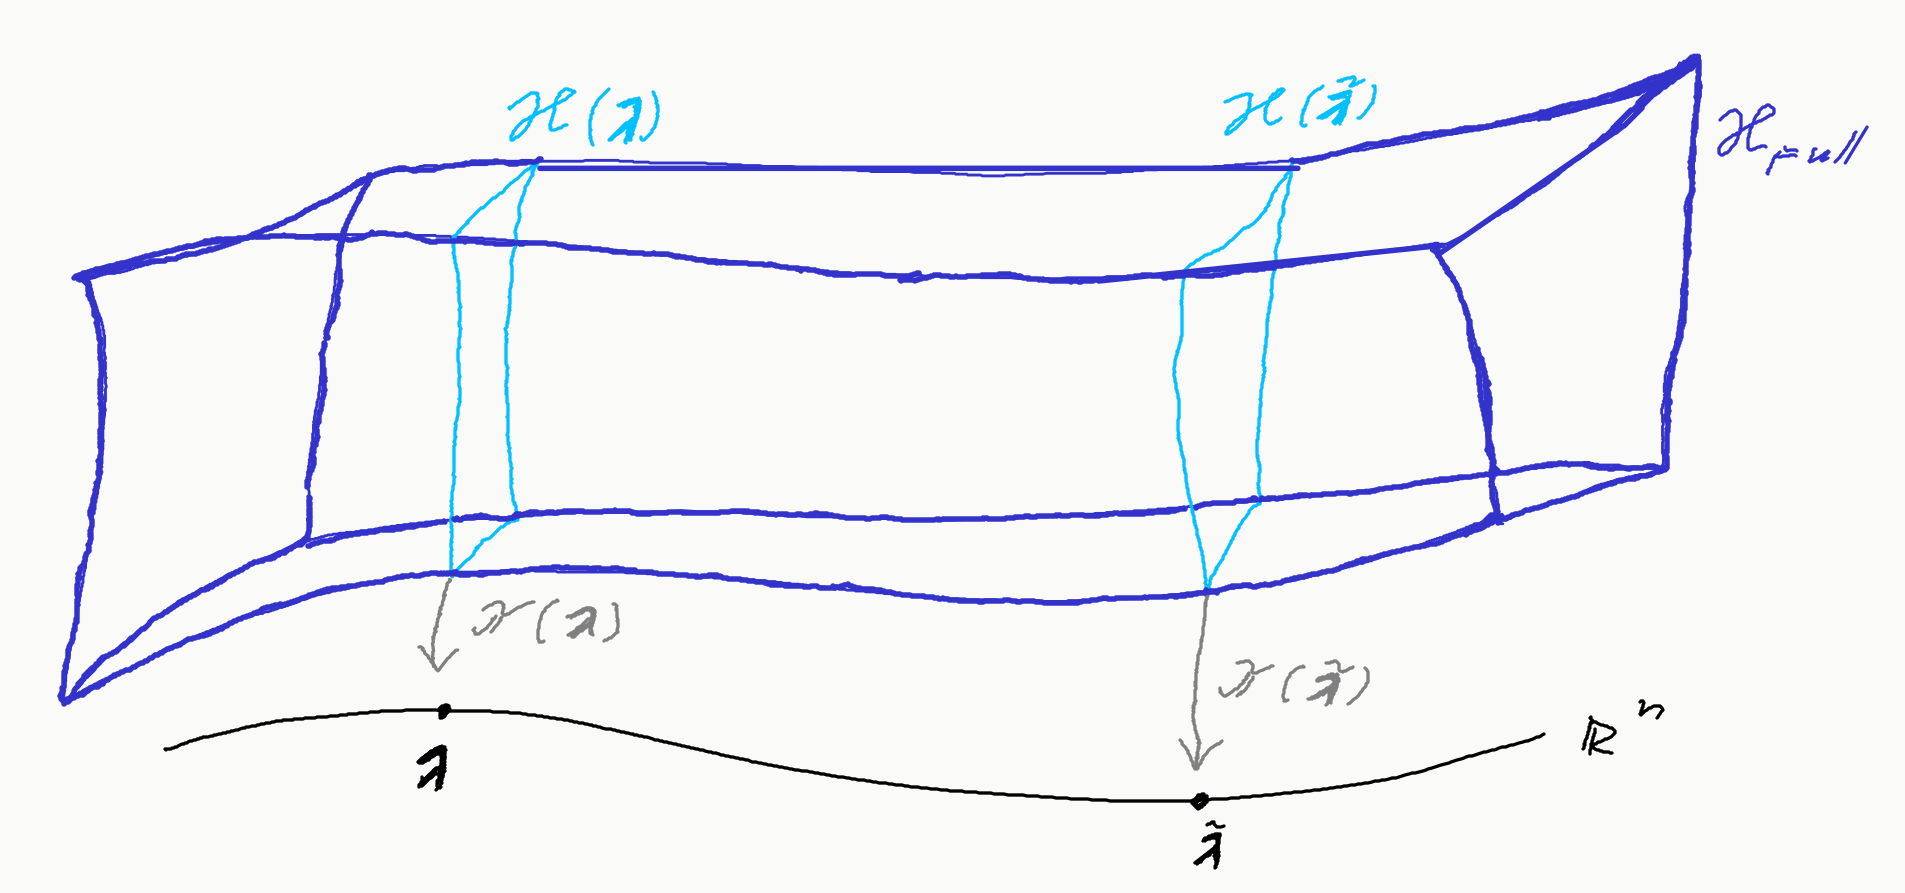
\includegraphics[width=\textwidth]{../img/manifold_basic.png}
\caption{Fiber bundle over $\R^n$ with Hilbert spaces $\H(\llambda)$ as individual fibers.}
    \label{fig:wholeBundle}
\end{figure}


Because we are interested only in discrete part of spectrum\footnote{Spectrum of the operator consists of discrete spectrum, calculable as eigenvalue problem, continuous and residual spectrum.}, it will further on be referred to only as \emph{spectrum}. 

The states of the system evolve according to the \Schrodinger equation
\begin{equation}
    i\hbar \d_t\kpsilt = \HH(\lambda)\kpsilt,
    \label{eq:schrodinger}
\end{equation}
which for eigenstates of instantaneous Hamiltonian reads as energy \Schrodinger equation
\begin{equation}
    \HH(\lambda)\ket{s(\lambda)}=E_s(\lambda)\ket{s(\lambda)}.
    \label{eq:energySchrodinger}
\end{equation}
For every $\H(\llambda)$ the first $k$ energies can be sorted from the lowest to create discrete set $\sigma(\HH(\llambda))\equiv\{E_0,\dots,E_k\}$. Clearly, there exists a bijection between all fibers $\H(\llambda)$, thus we can define \emph{section} $\mathrm{sec}_s$, mapping eigenstate corresponding to energy $E_s$ to base manifold 
$$\mathrm{sec}_s: \ket{o(\llambda)}\mapsto \mathcal{U}\subset \R^n,$$
which is also bijection. For $\forall s\in\{0,k\}$ we can create according to sec. \ref{sec:section} new \emph{energy manifolds}
$$\M_s\subset \M,$$
with special importance of the \emph{ground state manifold} $\M_0$, which will be used later on for adiabatic transports of ground states. Geometrical intuition is drawn on fig. \ref{fig:fullStructure}. Because those manifolds were created by sectioning, they are considered to be vector spaces in a geometrical sense. This was expected, because they contain quantum states.

\begin{figure}[h]
    \centering
    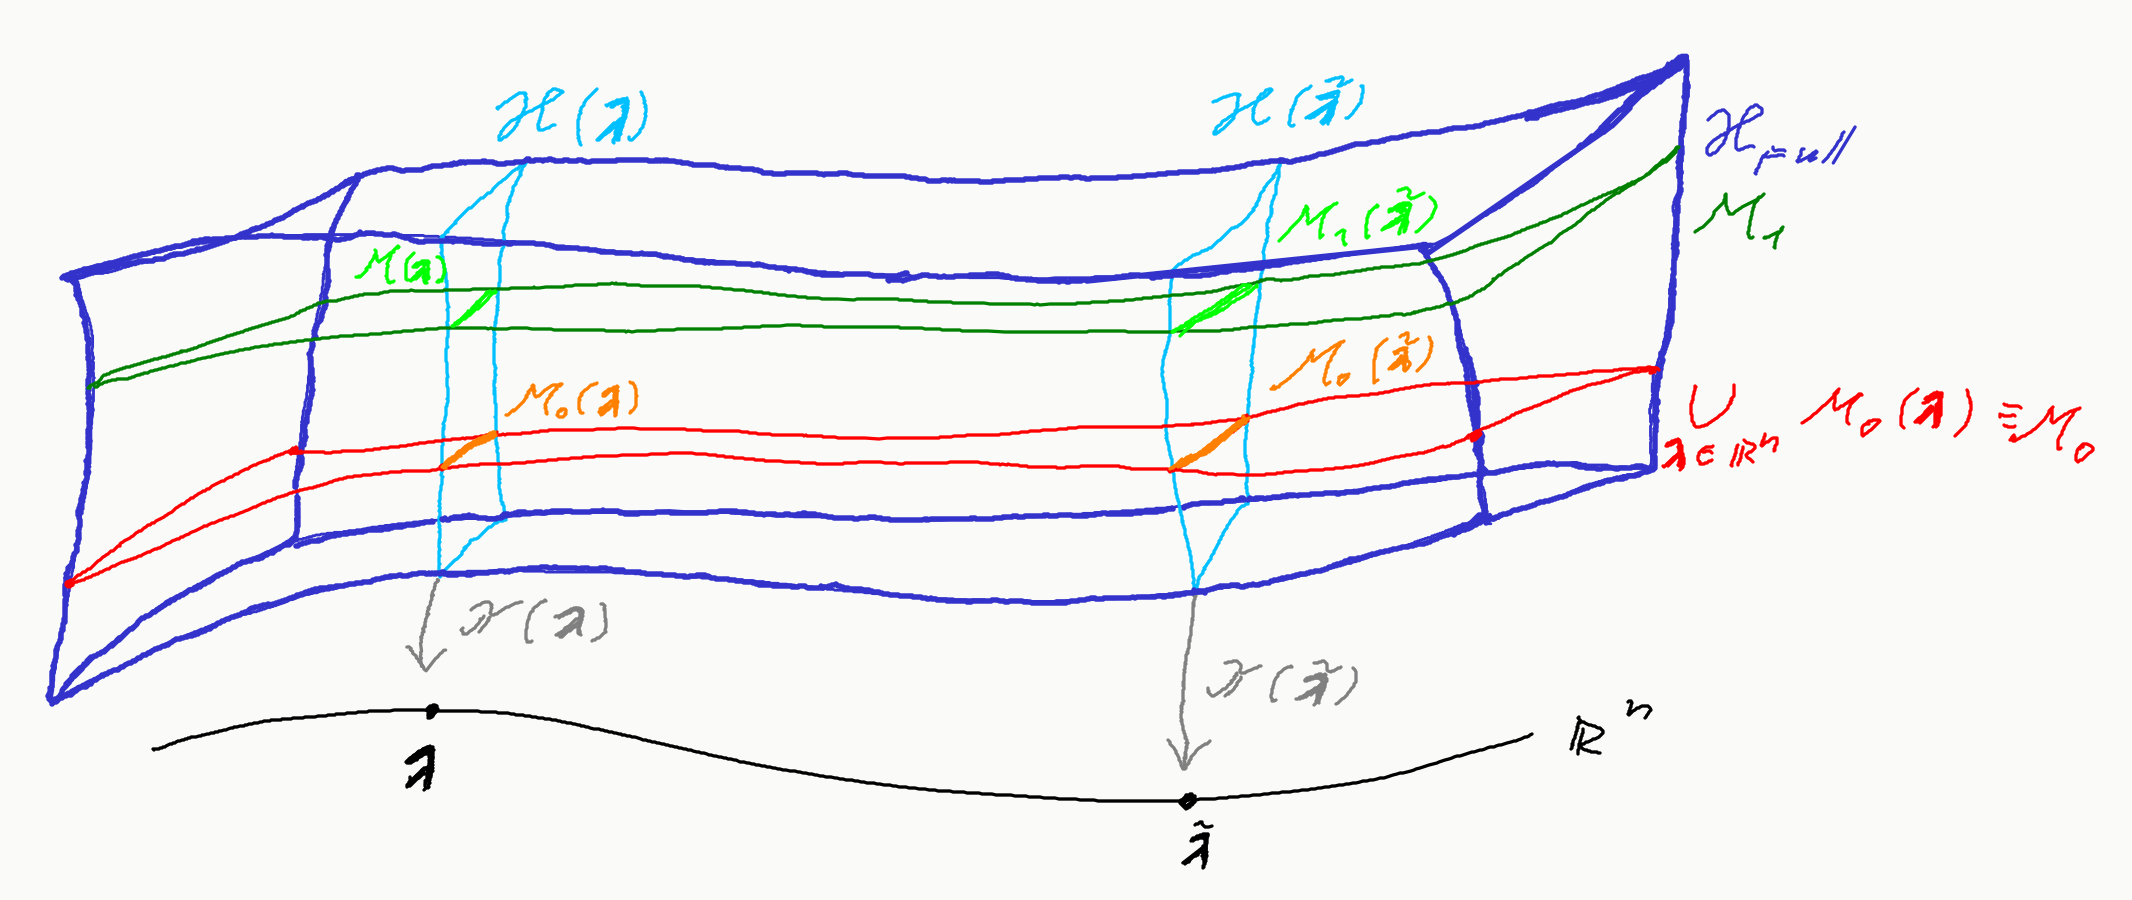
\includegraphics[width=\textwidth]{../img/manifold_full.png}
\caption{Geometrical intuition to transport on fiber manifold sections $\M_i$.}
    \label{fig:fullStructure}
\end{figure}




All Hilbert spaces above are considered to be spaces of \emph{bare states} $\H$. In quantum mechanics, physical observables are related to the \emph{space of rays}, defined as $\P\H\coloneqq \H/U(1)$, where elements of $U(1)$ are unitary transformations $e^{i\phi}$ for $\phi\in\R$ defining gauge symmetry between quantum states. The geometrical intuition is drawn for any $\llambda$ on fig. \ref{fig:projectiveHilbertSpace}.
\begin{figure}[h]
    \centering
    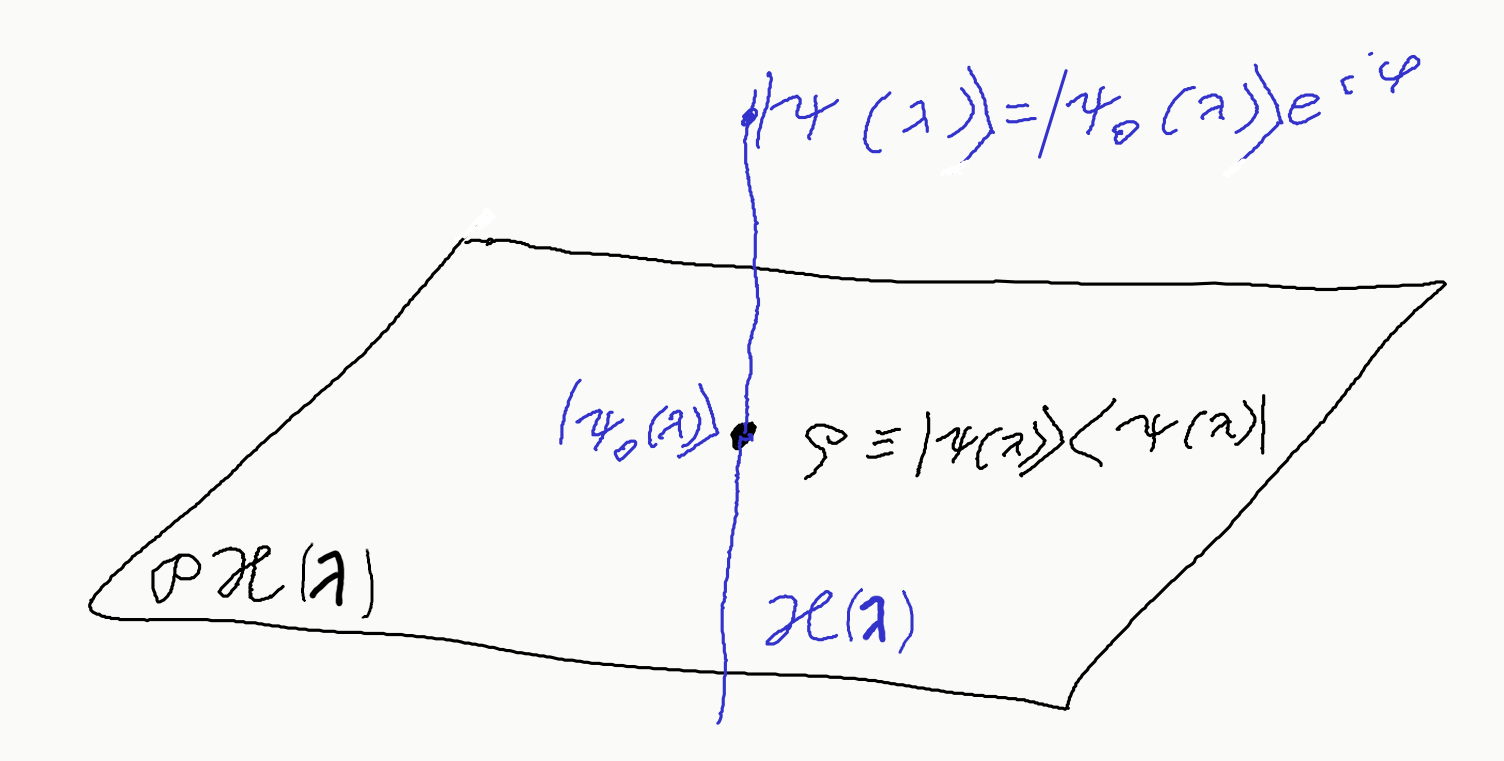
\includegraphics[width=0.8\textwidth]{../img/projectiveHilbertSpace.png}
\caption{Space of bare states and its projection to space of rays $\P\H(\llambda)\coloneqq \H(\llambda/U(1)$.}
    \label{fig:projectiveHilbertSpace}
\end{figure}

This means, that energy manifolds $\M_s$, generated by bare states, are again of fiber structure, defined as
$$\left(\H,\P\H,\pi_{rays},\{e^{i\phi}\ket{\psi} \text{ for }\phi\in\R\}\right),$$
where $\pi_{rays}$ is just rule setting phase $\phi$ to zero. Because ll $\M_s$ are compact and connected, they are diffeomorphic to each other.


\section{Transporting states}
Let's now focus on decomposition of $\H_{full}$ to different state manifolds $\M_s$, as displayed on figure \ref{fig:manifoldCutIntuition}.

\begin{figure}[h]
    \centering
    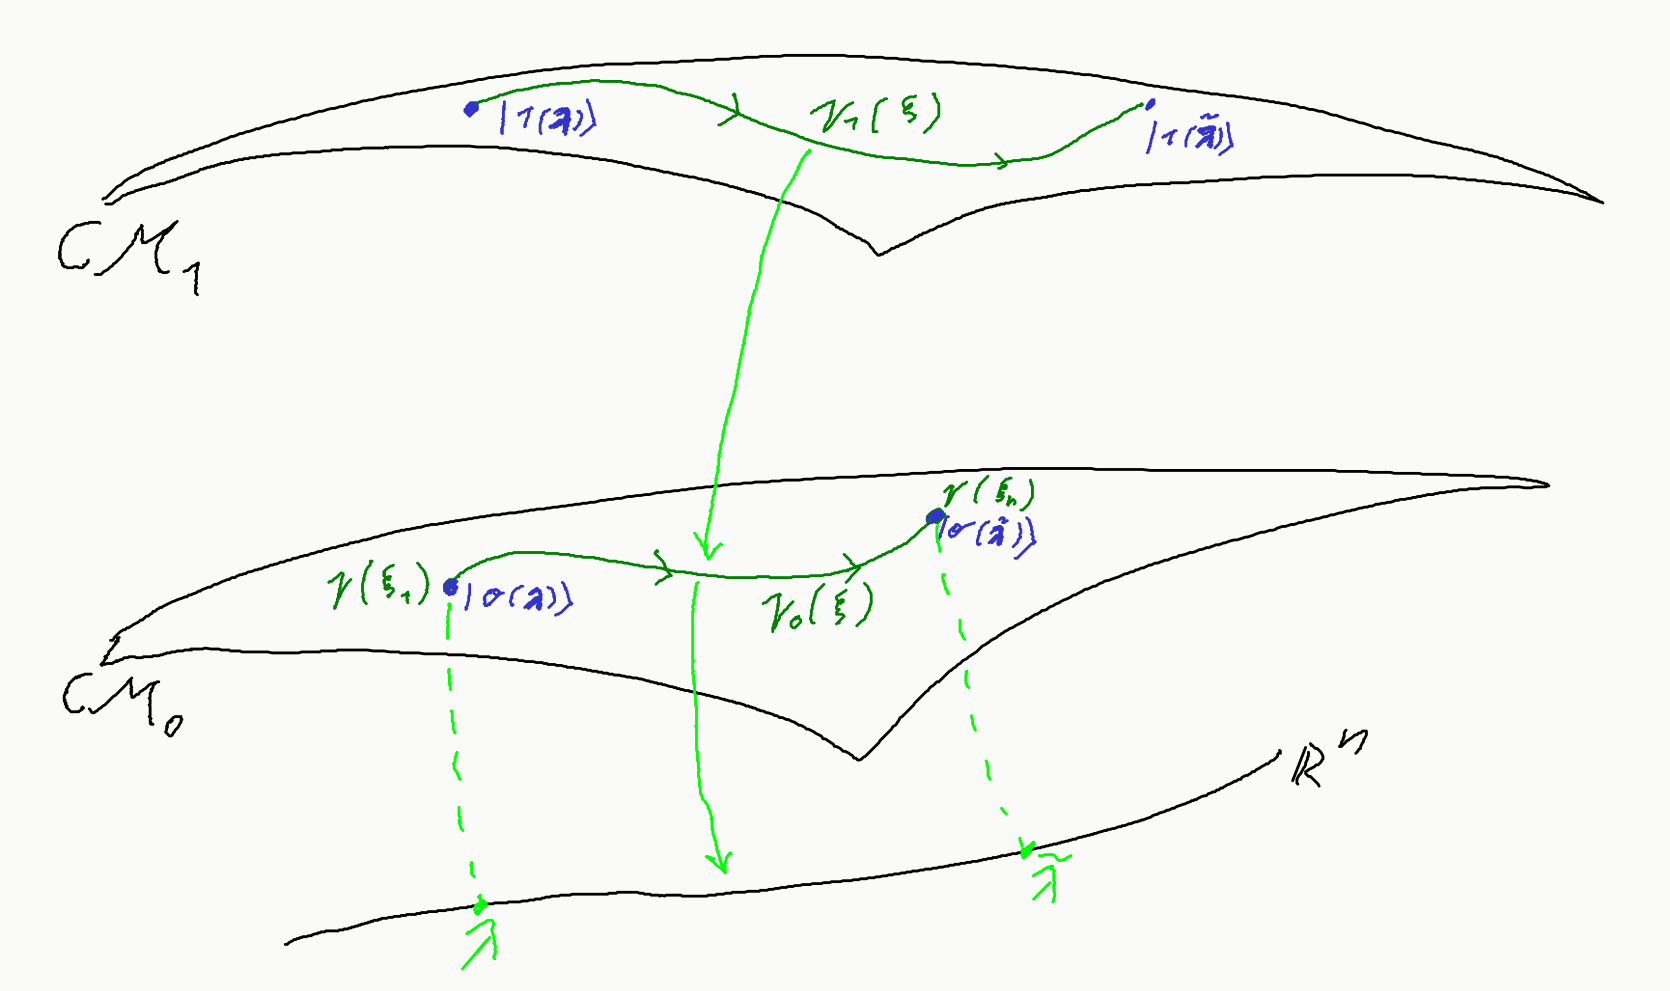
\includegraphics[width=\textwidth]{../img/manifoldCutIntuition.png}
\caption{Geometrical intuition to transport on fiber manifold sections $\M_s$.}
    \label{fig:manifoldCutIntuition}
\end{figure}

Changing state from eigenstate $\ket{s(\llambda)}$ to any pure state $\ket{\psi(\tilde\llambda)}$, during some time period, is unitary transformation and can be thought of as \emph{parallel transport on fiber bundle} between two vectors. Assuming the transport goes along curve $\{\gamma_s(\xi)|\xi\in[\xi_1,\xi_2]\subset \R\}\subset \M_s$ This can be written as
\begin{equation}
    \kpsit \equiv \Par_{\gamma_s}\ket{s(\lambda)} = \exp\left(-\frac{i}{\hbar}\int_0^tE_s(\tau)\d\tau)\right)\exp(i\gamma_s(\xi))\ket{s(\lambda)}.
    \label{eq:phasesOnManifold}
\end{equation}
The first exponential, the \emph{dynamical phase}, is well known solution to energy \Schrodinger equation \ref{eq:energySchrodinger} with $\llambda=const$ and depends only on time and energy of states during the transport. The second exponential is called \emph{geometrical phase}. This phase is generally non-integrable, meaning it cannot be written simply as $\gamma_s(\lambda)$ and for some closed curve on $\M$
\begin{equation}
    C=\{\llambda(\xi)|\xi\in[0,\Xi] \text{, such that }\llambda(0)=\llambda(\Xi)\}
\end{equation} 
we generally get $\Par_C \ket{\psi(\llambda)}\neq \ket{\psi(\llambda)}$. This property is sometimes more generally called an \emph{anholonomy} % and should be defined properly.
% \begin{definition}[Anholonomy]
%     Geometrical phenomenon, which causes some variable $V(\gamma(p))$ not to return to it's original value while varying it's parameter $p$ around some closed curve $\gamma(p)$. 
% \end{definition}
and geometric intuition can be seen on fig. \ref{fig:parallelTransportClosed}.
\begin{figure}[h]
    \centering
    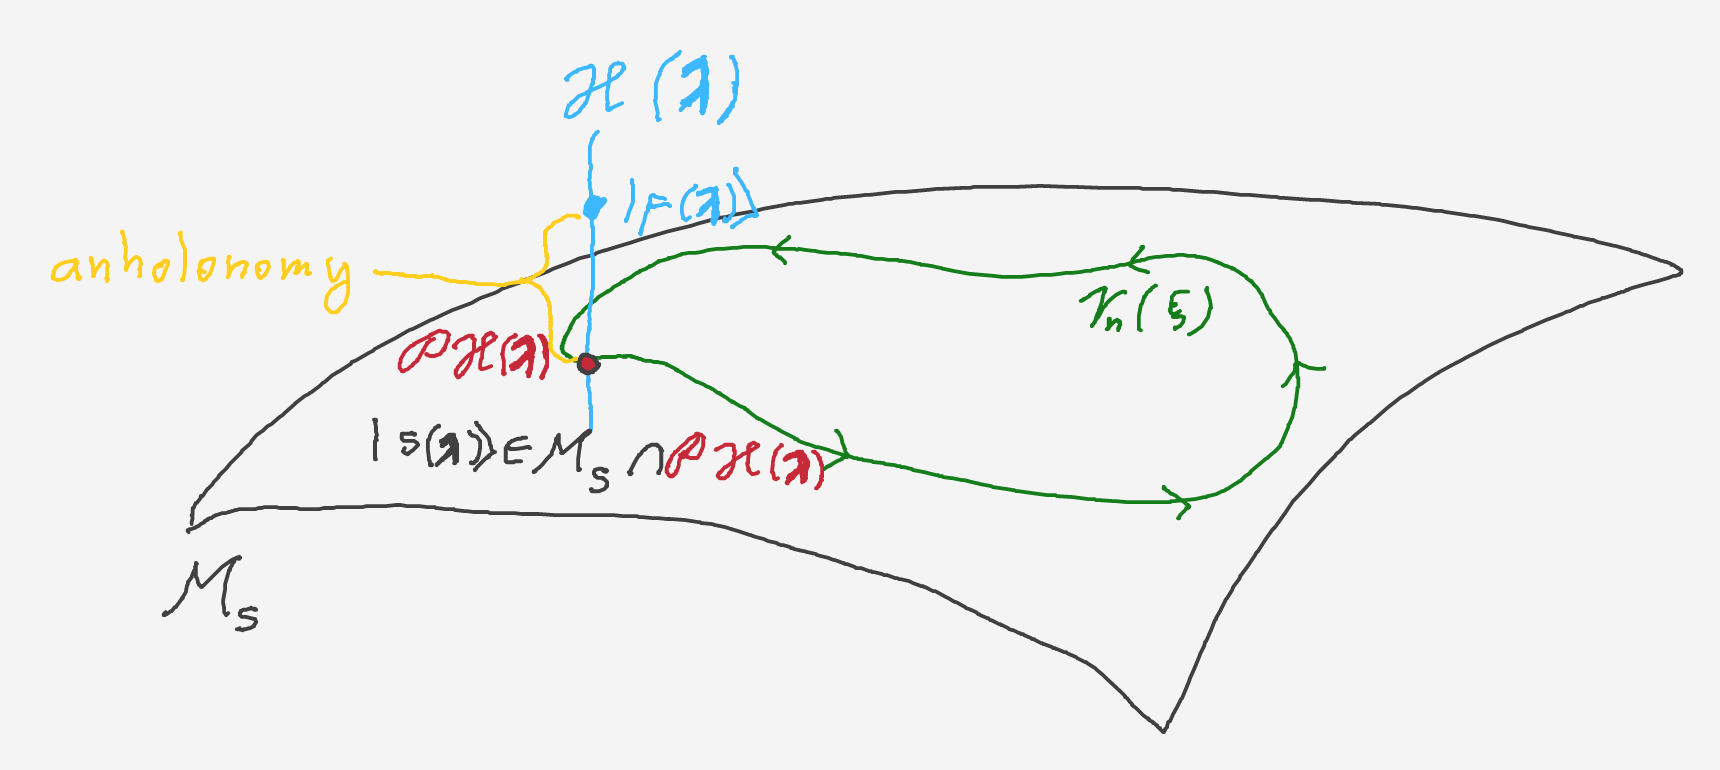
\includegraphics[width=0.8\textwidth]{../img/parallelTransportClosedCurve.png}
\caption{Parallel transporting around some closed curve $C$ with anholonomy drawn in yellow.}
    \label{fig:parallelTransportClosed}
\end{figure}

For quantum states, the anholonomy can be measured as a non-zero angle between $\ket{V}$ and $\Par_C\ket{V}$, meaning
$$\braket{V|\Par_C|V}\neq 0.$$ 


Substituting general solution \ref{eq:phasesOnManifold} to eq. \ref{eq:schrodinger} yields (see \citep{berry1984})
\begin{equation}
    \d_t \gamma(\lambda)=i\braket{s(\lambda)|\partial_\mu s(\lambda)} \d_t \lambda^\mu(\lambda).
\end{equation}
Integrating this equation around some closed curve $C$ and assuming the dynamical phase to be zero, thus not exciting the system, we get
\begin{equation}
    \gamma_n(C)=i\oint_C\braket{s(\llambda)|\partial_\mu s(\llambda)}\d \lambda^\mu.
    \label{eq:gammaCoint}
\end{equation}
We see, that the geometric phase does not depend on energy or time, only on the sequence of Hamiltonians, which means it depends only on the path itself.




The problem of expressions above lies in $\partial_\llambda s(\llambda)$, which locally requires knowledge of single-valued basis $\{\ket{0},\dots, \ket{k}\}$. This can be avoided in 3-dimensions using Stokes's theorem for $S$ as the surface with boundary $\partial S=C$, for coordinate gradient $\nabla$
\begin{equation}
    \begin{split}
        \gamma_s(C) &= -\Im \iint_C \d S \cdot \nabla \times \braket{s(\llambda)|\nabla n(\llambda)}\\
         &= -\Im \iint_C \d S \cdot \braket{\nabla s(\llambda)|\times|\nabla s(\llambda)}\\
        &= -\Im \iint_C \d S \cdot \sum_{m\neq s} \braket{\nabla s(\llambda)|m(\llambda)}\times \braket{m(\llambda)|\nabla s(\llambda)}\\
        &= -\iint_C \d S \cdot V_s(\llambda)
            \label{eq:stokes}
    \end{split}
\end{equation}
for 
\begin{equation}
    V_s(\llambda) = \Im \frac{
            \braket{s(\llambda)\nabla_\llambda \HH(\llambda) |m(\llambda)}\times \braket{m(\llambda)|\nabla_\llambda \HH(\llambda)|s(\llambda)}    
             }{
(E_m(\llambda)-E_s(\llambda))^2
            }
\end{equation}
where the element of summation $m=s$ in third step of derivation is real, therefore has no influence on $\gamma_s$ and can be omitted. The last equivalence holds, because if we differentiate the \Schrodinger equation \ref{eq:energySchrodinger}, we get for any $\ket{s},\ket{m}\in \M$
\begin{equation}
    \begin{split}
        \nabla \HH\ket{s(\llambda)}+\HH \ket{\nabla s(\llambda)} &= E_s\ket{\nabla s(\llambda)}\\
        \braket{m(\llambda)|\nabla \HH|s(\llambda)}+\braket{m(\llambda)|E_m|\nabla s(\llambda)} &= \braket{m(\llambda)|\nabla \HH|s(\llambda)}\\
        \braket{m(\llambda)|\nabla s(\llambda)}&=
        \frac{\braket{m(\llambda)|\nabla \HH |s(\llambda)}}
        { E_m(\llambda)-E_s(\llambda)}, \qquad s\neq m,
    \end{split}
\end{equation}
where we used $\ket{\nabla s}\equiv\nabla \ket{ s}$.
Comparing the first expression in eq. \ref{eq:stokes} with its last one and extending it to real numbers, we get
\begin{equation}
    V_s(\llambda)=\nabla\times\braket{s(\llambda)|\nabla m(\llambda)}, 
    \label{eq:vectorPotentialDef}  
\end{equation}
defining vector potential of $V_s(\llambda)$. In addition, it extends our definition from single valued basis to any solution of \ref{eq:energySchrodinger}, thus instead of ground state manifold, we can use any $\M_s$.

As was mentioned, the above procedure from eq. \ref{eq:gammaCoint} was performed only for three-dimensional space. Proper generalization to n-dimensional space would yield, see \citep{berry1984},
\begin{equation}
    \gamma_s(C) = -\iint_C \d S \cdot\Im \frac{
            \braket{s(\llambda)\d \HH(\llambda) |m(\llambda)}\wedge \braket{m(\llambda)|\d\HH(\llambda)|s(\llambda)}    
             }{
(E_m(\llambda)-E_s(\llambda))^2
             },
\end{equation}
which will not be needed in this thesis.




\section{Metric and geometric tensor}
As a playground for this chapter, we will choose the ground state manifold $\M_0$, but it can be easily generalized to any energy states manifold $\M_s$. From now on we will use natural units, so $\hbar=1$.
% Our first guess might be
% \begin{equation}
%     \d \tilde{s}^2 = \braket{i(\bm\llambda+\d\bm\llambda)|i(\bm\llambda+\d\bm\llambda)} = 1-2\Re{\braket{i(\bm\llambda+\bm\d\llambda)|i(\bm\llambda)}}.
% \end{equation}
% This is \emph{gauge dependent}, meaning that it depends on our choice of the wave phase, i.e. on observer. 

Let's first look at $\P\M_s$, which is needed to be \emph{gauge independent}. Gauge dependence in quantum mechanics means, that the change in phase factor $\phi$ of some state $\ket{o(\llambda)}\in \T_\llambda\M$ induces the change 
\begin{equation}
    \ket{o(\llambda)}\mapsto e^{i\phi(\llambda)} \ket{o(\llambda)} \implies \braket{o(\llambda)|\nabla o(\llambda)}\mapsto \braket{o(\llambda)|\nabla o(\llambda)} + i\nabla \phi(\llambda) 
\end{equation} 
For $\phi(\llambda)\in \mathcal C^2$ we see from eq. \ref{eq:vectorPotentialDef}, that gauge independent choice would be for infinitesimal change for example
\begin{equation}
    f=\braket{o(\bm\llambda+\delta\bm\llambda)|o(\bm\llambda)},
\end{equation}
sometimes referred to as the \emph{fidelity of a ground state}\footnote{Generalization for any mixed state is for two density matrices $\sigma$, $\rho$ as $$f\coloneqq \left(\Tr \sqrt{\sqrt{\rho}\sigma\sqrt{\rho}}\right)$$}. We can see it's physical meaning imagining \emph{quantum quench} (rapid change of some Hamiltonian parameters), in which case $f^2$ is the probability that system will remain in the new ground state. $1-f^2$ is therefore probability of exciting the system during this quench, which leads to the definition of \emph{distance on $\M_0$}\footnote{$\d$ notation is in differential geometry assumed to be an exterior differential. On functions, it acts as $\d: \F\M\rightarrow \mathcal{T}_1\M$ and intuitively corresponds to total differential from functional analysis.}
\begin{equation}
    \d s^2 \equiv 1-f^2= 1-\left|\braket{o(\bm\llambda+\delta\bm\llambda)|o(\bm\llambda)}\right|^2.
    \label{eq:distanceOnM0}
\end{equation}
We can easily check, that the axioms of metric defined using distance as bilinear form $s$ between elements $\kpsi,\; \kphi\in \M_0$ are for \textcolor{red}{closed systems} satisfied:
\begin{itemize}
    \item identity of indiscernibles $s(\kpsi,e^{i\alpha}\kpsi) = 0 \Leftrightarrow \kpsi=\kphi$, $\alpha\in\R$,
    \item symmetry for any two states $\kpsi$, $\kphi$ is implied by $|\braket{\psi|\phi}|=|\braket{\phi|\psi}|$
    \item triangle inequality: $s(\kpsi,\ket{\psi_2}) <s(\kpsi,\kpsi_1) + s(\ket{\psi_1},\ket{\psi_2})$ for any $\ket{\psi_1}$.
\end{itemize}
Because $1-f^2>0$, the first term of Taylor expansion is zero, thus we have for a metric tensor
\begin{equation}
    \d s^2 = g_{\mu\nu}\d \lambda^\mu \d\lambda^\nu+\O(\lambda^3).
\end{equation} 

Let's define the metric on the space of states $\M_0$ and then see, how it corresponds to fidelity. This metric is called the \emph{Geometric tensor}, and can be expressed as 
\begin{equation}
    \chi_{\mu\nu}\coloneqq \braket{\partial_\mu o|\partial_\nu o}_c \equiv \braket{\partial_\mu o|\partial_\nu o} - \braket{\partial_\mu o|o}\braket{o|\partial_\nu o},
    \label{eq:geometricTensor}
\end{equation}
where shortened notation $\partial_\nu\coloneqq\pder{}{\lambda^\nu}$ was used.
Because $\chi$ is Hermitian ($\chi_{\mu\nu}=\chi^*_{\nu\mu}$), only the symmetric part determines the distance between states
\begin{equation}
    \d s^2= g_{\mu\nu}\d \lambda^\mu \d\lambda^\nu= \chi_{\mu\nu}\d \lambda^\mu \d\lambda^\nu,
\end{equation}
therefore it is practical to decompose it as
\begin{equation}
    \chi_{\mu\nu} \equiv g_{\mu\nu} - i\frac{1}{2} \nu_{\mu\nu},
\end{equation}
where the \emph{Fubini-Study tensor}\footnote{In some literature, this is called Geometric tensor}, as it's called, is metric on $\P\M_0$ and can be expressed as
\begin{equation}
    g_{\mu\nu} = \frac{\chi_{\mu\nu}+\chi_{\nu\mu}}{2} = \Re\braket{\partial_\mu o|\partial_\nu o}_c = \Re \sum_{o\neq j}\frac{\braket{o|\pder{\H}{\lambda^\mu}|j}\braket{j|\pder{\H}{\lambda^\nu}|o}}{(E_o-E_j)^2},
    \label{eq:metrictensorREdefinition}
\end{equation}
and the \emph{curvature tensor} a.k.a. \emph{Berry curvature} is
\begin{equation}
        \nu_{\mu\nu} = i(\chi_{\mu\nu}-\chi_{\nu\mu})= \Im\braket{o|[\overleftarrow{\partial}_\nu,\partial_\mu]|o}_c = -2 \Im \sum_{o\neq j}\frac{\braket{o|\pder{\H}{\lambda^\mu}|j}\braket{j|\pder{\H}{\lambda^\nu}|o}}{(E_o-E_j)^2},
    \label{eq:geom.tensorREdefinition}
\end{equation}
where $\overleftarrow{\partial}_\nu$ affects the covector on the left.


\section{Derivation of the geometric tensor}
\label{sec:derivationOfGeometricTensor}
To prove the correspondence of geometric tensor, described by eq. \ref{eq:geometricTensor}, to distance on $\M_0$, see eq. \ref{eq:distanceOnM0}, we start with eigenstate $\ket{o(\llambda)}\in \M_0\cap \H(\llambda)$. Changing parameters $\llambda$ to $\llambda+\delta \llambda$ results in Hamiltonian $\HH_f$ with eigenstates $\ket{s(\llambda+\delta \llambda)}\in \M_s\cap\H(\llambda+\delta \llambda)$, meaning it can be excited. Probability amplitude of going to such state is
\begin{equation}
    \begin{split}
        a_s&=\braket{s(\llambda+\delta\llambda)|o(\llambda)}\approx \delta\lambda^\mu\braket{\partial_\mu s(\llambda)|o(\llambda)} \\
        &= -\delta\lambda^\mu\braket{s(\llambda)|\partial_\mu|o(\llambda)}.
    \end{split}
\end{equation}

If we introduce the \emph{gauge potential}, aka \emph{calibration potential}, as\footnote{In SI units, the gauge potential is $\AA_\mu\equiv i\hbar\partial_{\mu}$}
\begin{equation}
    \AA_\mu\equiv i\partial_{\mu},
\end{equation}
the probability amplitude can be expressed as
\begin{equation}
   a=i\braket{s(\llambda)|\AA_\mu |o(\llambda)}\delta\lambda^\mu,
   \label{eq:probabilityOfTransitionIsGauge}
\end{equation}
which has meaning of matrix elements of the gauge potential. Probability of the excitation i.e. transition to any state $s>0$ from ground state is then (omitting the $\llambda$ dependence in notation)
\begin{equation}
    \begin{split}
        \sum_{s\neq 0}|a_s|^2&=  \sum_{s\neq 0} \delta \lambda^\mu \delta \lambda^\nu\braket{o|\AA_\mu|s}\braket{s|\AA_\nu|o}+\O(|\delta \lambda^3|) \\
        &= \delta \lambda^\mu \delta \lambda^\nu\braket{o|\AA_\mu \AA_\nu|o}_c\eqqcolon \delta \lambda^\mu \delta \lambda^\nu\chi_{\mu\nu}+\O(|\delta \lambda^3|),
    \end{split}
\end{equation}
where last term defines the geometric tensor.

\textcolor{red}{The gauge transformation means, that if the fidelity $f<1$, this potential can be subtracted from the Hamiltonian leading to $f=1$. This will be discussed later on in chapter \ref{chap:gauge}.}


\newpage





\section{Adiabaticity}
Adiabatic transformation is such a transformation from $\M$ to $\M$, which does not excite the system, meaning the fidelity $f=1$. Generally it can be achieved by two ways -- infinitely slow transformation of states, or adding some \emph{counter-diabatic elements} to the Hamiltonian to counter the excitation.


In this chapter, we will be dealing with the system described by the finite-dimensional Hamiltonian $\HH(\llambda)$ which drives the system according to \Schrodinger equation from some initial state $\ket{s(\llambda}$ to $\ket{s(\tilde\llambda)}$ along some path. Again we reduce the dimension from $\R^n$ to $1$ prescribing the curve $\gamma(\lambda)$ parametrized by time $t$, so we get $\HH=\HH(\lambda)$. Before going throw the details of adiabatic transformations, let's define its meaning properly.

\begin{definition}[Adibaticity]
    Slow change of parameters driving Hamiltonian in a sense, that it does not excite the system and allows the system to return to the same energetic state after circulation around any closed path on the manifold with fidelity $f=1$. For more see Theorem \ref{adiabaticTheorem}.
\end{definition}


\subsection{Slow transports}
\citep{kolodrubez}[chap. 2.3]
As was mentioned in the introduction to this chapter, one way to change the system parameters without exciting it is to change the driving parameter slowly enough. The meaning of the word "slow" clears up next theorem.
\begin{thm}[Adiabatic theorem]
    \label{adiabaticTheorem}
    For Hamiltonian $\HH$ varying in the time range $T$, the solution of the Schrödinger equation 
    $$\HH(\lambda)\ket{\psi_n(\lambda)} = E_n(\lambda)\ket{\psi_n(\lambda)}$$
    with initial condition in x-representation $\braket{x|\psi(t=0}=\psi_n(x,0)$ can be approximated as
    \begin{equation}
      ||\psi(\lambda) - \psi_{ad}(\lambda)||\approx o\left(\frac{1}{T}\right)
    \end{equation}
    for \emph{adiabatic state}
    \begin{equation}
        \ket{\psi_{ad}}= e^{\theta_n(\lambda)}e^{\gamma_n(\lambda)}\ket{\psi(\lambda)},
    \end{equation}
    where we define \emph{nongeometrical phase} induced by energy transitions,
    $$\theta_n(\lambda)\equiv -\frac{1}{\hbar}\int_0^t E_n(\tau)\d \tau$$
    and \emph{geometrical phase}, also called \emph{Berry phase}
        $$\gamma_n(\lambda)\equiv \int_0^t \underbrace{i\braket{\psi_n(\tau)|\partial_t\psi_n(\tau)}}_{\nu_n(\tau)} \d \tau .$$
\end{thm}
\begin{myproof}
    TBD (na wiki je)
\end{myproof}
Assume differentiable and non-singular Hamiltonian $\HH(\llambda)$ with degenerate basis $\{\ket{m,\llambda}\}_m$ called the \emph{adiabatic basis}. This is generally the family of adiabatically connected eigenstates\footnote{In the case of energy level crossing, the eigenstates are not unified, because transition between them is not adiabatical.} The transition amplitude between states for adiabatic change is
\begin{equation}
    0=\bra{m(\llambda)}\HH\ket{n(\tilde\llambda)} \quad \text{for }n\neq m, \forall \llambda,\forall \tilde \llambda.
\end{equation}
This can be driven along some curve $\gamma(\lambda)$, i.e. differentiated by $\partial_t$:
\begin{equation}
    \begin{split}
        0&=\bra{\partial_t m(\llambda)}\HH(\tilde \llambda)\ket{n(\tilde\llambda)}+ \bra{m(\llambda)}\overbrace{\partial_t\HH(\tilde \llambda)}^{\approx \partial_t\HH(\llambda)}\ket{n(\tilde\llambda)}+ \bra{m(\llambda)}\HH(\tilde \llambda)\ket{\partial_t n(\tilde \llambda)}\\
        &=E_n(\lambda)\braket{\partial_t m(\llambda)|n(\tilde \llambda)} + E_m(\lambda)\braket{m(\llambda)|\partial_t n(\tilde \llambda)}+ \bra{m(\llambda)}\partial_t \HH(\tilde\llambda)\ket{n(\tilde \llambda)}\\
        &= (E_m(\lambda)-E_n(\lambda))\underbrace{\braket{m|\partial_t (\tilde \llambda)}}_{-\frac{i}{\hbar}\bra{m}\AA_t\ket{n(\tilde \llambda)}} + \braket{m|\partial_t\HH|n(\tilde \llambda)}.
    \end{split}
\end{equation}
\textcolor{red}{
In matrix form, we can rewrite this equation as
\begin{equation}
    i\hbar\partial_t\HH=[\AA_t,\HH]-i\hbar \hat{M}_t\qquad \text{for } \hat{M}_t\equiv -\sum_n\pder{E_n(\lambda)}{t}\ket{n(\lambda)}\bra{n(\lambda)}.
\end{equation}
$\hat{M}$ is diagonal in energetic basis and it's elements has meaning of \emph{generalized force}, which correspond to corresponding energetic states. We can easily see that $[\HH,\hat{M}]=0$, implying
\begin{equation}
    [\HH,i\hbar\partial_t\HH-[\AA_t,\HH]]=0.
    \label{eq:komutation}
\end{equation}
This can be used as the definition for \emph{counter-diabatic potential} $\AA_t$. The strength of this equation lies in the fact, that it finds counter-diabatic potential without the need of Hamiltonian diagonalization.}


\section{Geodetic driving}
\label{chap:gauge}

\section{Gauge potentials}
In section \ref{sec:derivationOfGeometricTensor} we introduced the gauge potential without proving its gauge meaning, but only stating its correspondence to transition probability, see eq. \ref{eq:probabilityOfTransitionIsGauge}.
\textcolor{red}{
\emph{Gauge transformations}, in classical mechanics called \emph{canonical}, can be defined such, that they preserve Lagrangian of the system under local transformations from some Lie group.} This implies, that gauge transformed Hamiltonian $\H(\llambda)$ and $\H(\llambda+\d \llambda)$ commutes with its canonically transformed version\footnote{This can be easily reformulated to the world of classical physics, where the commutator is replaced by Poisson bracket.} 
 \begin{equation}
     [\HH(\llambda),\HH(\llambda+\delta \llambda)]=0.
 \end{equation}

 To understand the meaning of gauge symmetries, let's first consider classical system and then move to quantum mechanics.


\subsection{Classical gauge potential}



In the Hamiltonian classical mechanics, we assume the manifold $\M$ part of the phase space defined using Hamiltonian $H=H(p_i,q_i)$, where momentum $p_i$ and position $q_i$ are assumed to form the orthogonal basis of the phase space
\begin{equation}
    \{q^i,p_j\}=\delta^i_j,
    \label{eq:canonicalCommutationDelta}
\end{equation}
which also defines \emph{calibrational freedom} in their choice. \emph{Canonical transformations} then by definition preserve this formula. Using the \emph{Poisson bracket}, defined as
\begin{equation}
    \{A,B\}\coloneqq \pder{A}{q^j}\pder{B}{p_j}-\pder{B}{q^j}\pder{A}{p_j},
\end{equation}
we will examine continuous canonical transformations generated by gauge potential $\A_\lambda$
\begin{align}
        q^j(\lambda+\delta\lambda)&=q^j(\lambda)-\pder{\A_\lambda(\bm{p},\bm{q})}{p_j}\delta\lambda \;\Rightarrow\; \pder{q^j}{\lambda}=-\pder{\A_\lambda}{p_j}=\{\A_\lambda,q^j\}
        \label{eq:gaugeAsGeneratorOfMotion1}\\
        p_j(\lambda+\delta\lambda)&=p_j(\lambda)-\pder{\A_\lambda(\bm{p},\bm{q})}{q^j}\delta\lambda \;\Rightarrow\; \pder{p_j}{\lambda}=-\pder{\A_\lambda}{q^j}=\{\A_\lambda,p_j\}.
        \label{eq:gaugeAsGeneratorOfMotion2}
\end{align}
Substituting this to relations of orthogonality \ref{eq:canonicalCommutationDelta}, we get
\begin{equation}
    \{q^j(\lambda+\delta\lambda),p_j(\lambda+\delta\lambda)\}=\delta^i_j + \mathcal{O}(\delta\lambda^2).
\end{equation}
 
If $\lambda$ is time parameter and $\A_t=-H$, equations \ref{eq:gaugeAsGeneratorOfMotion1},\ref{eq:gaugeAsGeneratorOfMotion2} are identical to the Hamilton equations
\begin{equation}
\begin{split}
    \dot{q}^j&=-\{H,q^j\} = \pder{H}{p_j}\\
    \dot{p}_j&=-\{H,p_j\} = -\pder{H}{q^j}.
\end{split}
\end{equation}
Because the Hamiltonian is generator of the movement in the phase space $(\bm{q},\bm{p})$, we can interpret $\A_t$ as the generators of the movement on $\M$. Other specific choice might be $\lambda=X^i$, which gives us the momentum components $\A_{X^i}=p_i$.

Generally every gauge symmetry is generated by its gauge potential and corresponds to some conserved property, as theorem of Emma Nöether states.



\subsection{Quantum gauge potential}
\citep{kolodrubez}[chap. 2.2]
The role of Poison brackets in quantum mechanics is taken by commutators, canonical transformations are called \emph{unitary transformations} and calibration freedom is hidden in the choice of basis. Now let's find some special basis transformations $\U$ between initial system $S$ and the transformed $\tilde{S}$. Both of them describe the system with Hamiltonian $\HH(\llambda)$ with eigenstates $\ket{n(\llambda)}$ and eigenstate manifolds $\M_n\equiv \cup_\llambda \{\ket{n(\llambda)}\}$. 

From fiber structure goes\footnote{especially from the fact, that all spaces $\HH(\llambda)$ are isomorphic to each other}, that any state of $\HH(\llambda)$ for $\forall \llambda\in U\subset \R^n$ can be decomposed as
    \begin{equation}
    \ket{\psi(\llambda)}\equiv \sum_n \psi_n(\llambda)\ket{n}
\end{equation}    
for some coordinate independent basis $\{\ket{n}\}_n$.
Then there exist unitary transformation
\begin{equation}
    \U(\llambda): \tilde S\rightarrow S,\quad \U(\llambda)\ket{m(\llambda)}=\ket{n}.
    \label{eq:transformationU}
\end{equation}
% where scalar parameter $t$ is assumed to be changing along the path $\gamma(t)$, corresponding to situation on fig. \ref{fig:manifoldCutIntuition}. This satisfies
% \begin{equation}
%     i\hbar \partial_t \U(t)=\HH(t)\U(t)
%     \label{eq:schrodingerForU}
% \end{equation}
% for any point on $\tilde\gamma(t)$ and $\HH$ the full Hamiltonian of the system, along which the partial derivative is taken.


The wave function $\kpsi$ in $S$ can be decomposed using Schmidt decomposition\footnote{The Schmidt decomposition can be performed in finite dimension, or if the Hamiltonian is compact, which is not automatic in quantum mechanics. What's more, the Hamiltonian is usually not even bounded. Anyway, for simple systems with bounded energy we can assume so.}
\begin{equation}
    \ket{\psi(\llambda)} = \sum_{m,n}\psi_n(\llambda) \ket{m(\llambda)}\overbrace{\braket{m(\llambda)|n}}^{U_{mn}(\llambda)} =\sum_m \overbrace{\tilde{\psi}_m(\llambda)}^{\braket{m(\llambda)|\psi_n|n}}\ket{m(\llambda)},
\end{equation}
where $U_{mn}(\llambda)$ are matrix elements of unitary transformation $\U(\llambda)$. In this work, we will be interested only in the gauge transformations preserving energy of the system.


\subsection{Adiabatic gauge potential}

Adiabatic gauge potentials, sometimes just \emph{adiabatic potentials}, are generators of unitary transformations, so we can define them analogically to the classical case
\begin{equation}
    i\hbar\partial_\lambda \ket{\tilde{\psi}(\llambda)} = i\hbar \partial_\lambda\left(\U^+(\llambda)\ket{\psi} \right)= \underbrace{i\hbar\left(\partial_\lambda \U^+(\llambda)\right)\U(\llambda)}_{-\tilde{\AA_\lambda}}\ket{\tilde{\psi}(\llambda)}.
\end{equation}
The adiabatic potential $\tilde{\AA_\lambda}$ can be transformed to non-tilde system as
\begin{equation}
    \begin{split}
        \AA_\lambda&=\U(\llambda)\tilde{\AA_\lambda}\U^+(\llambda) = -i\hbar\U(\llambda)\big(\partial_\lambda \U^+(\llambda)\big) =\\
        &= -i\hbar\partial_\lambda\big(\underbrace{U^+(\llambda)U(\llambda)}_{\mathds{1}}\big)-\big(\partial_\lambda U(\llambda)\big)U^+(\llambda) \big) =i\hbar \big(\partial_\lambda U(\llambda\big)U^+(\llambda).
    \end{split}
\end{equation}
From this we get the equations for adiabatic potential in two systems
\begin{align}
    \AA_\lambda&=i\hbar \big(\partial_\lambda U(\llambda)\big)U^+(\llambda)
    \label{eq:adiabaticPotential}\\
    \tilde{\AA_\lambda} &= -i\hbar\left(\partial_\lambda \U^+(\llambda)\right)\U(\llambda)
    \label{eq:adiabaticPotentialTilde}
\end{align}
which can be shown to be Hermitian
\begin{equation}
     \tilde{\AA_\lambda}^+=i\hbar U(\llambda)^+\big(\partial_\lambda\U(\llambda)\big)=-i\hbar\big(\partial_\lambda\U(\llambda)^+\big)\U(\llambda) = \tilde{\AA_\lambda},
     \label{eq:counterdiabaticPotentialTwoSystems}
\end{equation}
analogically for non-tilde potential.
Using the eigenbasis of $\HH$, the matrix elements are
\begin{equation}
    \bra{n}\tilde{\AA_\lambda}\ket{m}=i\hbar\bra{n}\U(\llambda)^+\partial_\lambda\U(\llambda)\ket{m} = i\hbar\bra{n(\llambda)}\partial_\lambda\ket{m(\llambda)}.
\end{equation}
and because
\begin{equation}
    \bra{n(\llambda)}\AA_\lambda\ket{ m(\llambda)}= \bra{n}\tilde{\AA_\lambda}\ket{m},
\end{equation}
we get
\begin{equation}
    \AA_\lambda = i\hbar\partial_\lambda.
    \label{eq:adiabaticPotentialDefinition}
\end{equation}
% It's good to point out, that we were applying tilde operators to non-tilde states et vice versa. This can be justified only if we consider $\M$ big enough to contain all necessary states, which can be achieved during the transformation.



Adiabatic gauge transformations are  class of gauge transformations with fidelity $f=1$. This means, that if the system is driven by Hamiltonian $\HH(\llambda)$ with fidelity $f<1$, there exists such adiabatic potential $\A_\lambda$, that driving of the same system using $\HH-\A_\lambda$ has fidelity $f=1$.

The adiabatic gauge potentials can then be understood as affine connections defining the parallel transport on fiber bundle, if we define covariant derivative as
\begin{equation}
    D_\mu=\partial_\mu+i\AA_\mu,
\end{equation}
which yields $D_\mu\ket{\psi_n}=0$ for every eigenstate, which yields, that the transport of eigenvalues on $\M_0$ is parallel. $\AA_\mu$ is generally defined \ref{eq:adiabaticPotential}, which generally gives non-zero covariant derivative for states not belonging to $\M_0$. 

Finding of those potentials has many practical applications, so let's introduce one analytical procedure of finding them.





\section{Counter-diabatic driving}
\label{chap:CounterDiabaticDriving}
\citep{kolodrubez}[page 15--17] The main idea of a counter-diabatic driving is, that any excitation of the system can be countered by adding so called \emph{counter-diabatic potential} to the Hamiltonian. Consider again any eigenstate $\kpsit$ of the Hamiltonian $\HH=\HH(\lambda)$ driven along the curve $\gamma(\lambda(t))$ on $\M_0$ depending on time $t$, during which the fidelity $f\neq 0$. Because the system is not measured during the trip, it can't be stated if or if not it was excited, but the main goal here is to make fidelity zero, which is iff $\tilde\HH$ is diagonal. For diagonalizable Hamiltonian, there exist a transformation, see eq. \ref{eq:transformationU}, for which the fidelity will be zero. Such a transformation does not have to be unique, but we can choose any one of them. This can be seen more clearly from direct transformation of the Schrödinger equation. 

The Schrödinger equation
\begin{equation}
    i\hbar \der{}{t}\ket{\psi(\lambda)} = \HH(\lambda)\ket{\psi(\lambda)}
\end{equation}
can be transformed using 
\begin{equation}
    \U(\lambda)^+  \ket{\psi(\lambda)} = \ket{\tilde\psi(\tilde\llambda)},
    \label{eq:transformationUtimeDependentH}
\end{equation}
for which $\tilde\HH\coloneqq\U^+\HH\U$ is diagonal, leading to
\begin{align}
    i\hbar \der{}{t}(\U(\tilde\llambda)\ket{\tilde \psi(\tilde\llambda)}) &= \HH(\lambda)\U(\tilde\llambda)\ket{\tilde \psi(\tilde\llambda)} \\
    i\hbar \der{\lambda}{t}\partial_\lambda\U(\tilde\llambda)\ket{\tilde \psi(\tilde\llambda)} + i\hbar \U(\tilde\llambda)\der{}{t}\ket{\tilde \psi(\tilde\llambda)} &= \HH(\lambda)\U(\tilde\llambda)\ket{\tilde \psi(\tilde\llambda)}.
\end{align}

This can be rewritten using adiabatic potential from eq. \ref{eq:adiabaticPotentialDefinition}, using \emph{dot} notation for time derivatives and omitting the points in which the objects are evaluated, as
\begin{equation}
    i\hbar \der{}{t}\ket{\tilde\psi} = \left[\U^+\HH\U-\dot{\lambda}\tilde{\AA_\lambda}\right]\ket{\tilde\psi} = \left[\tilde \HH-\dot{\lambda}\tilde{\AA_\lambda}\right]\ket{\tilde{\psi}} \eqqcolon \tilde{\HH}_m \ket{\tilde{\psi}},
\end{equation}
where the term $-\dot{\lambda}\tilde{\AA_\lambda}$ is called \emph{Galilean} and $ \tilde{\HH}_m$ is the Hamiltonian in transformed system. Because $\tilde{\HH}$ is diagonal, it drives $\ket{\tilde{\psi}}$ with fidelity $f=1$. This means that for any driving defined by $\HH(\lambda(t))$, which defines the unitary transformation $\U$, there exists such \emph{counter-diabatic potential} $\AA_\lambda$, that $\HH_m + \dot{\lambda}\AA_\lambda$ has $f=1$.


% Intuition for transformations using original Hamiltonian vs. transformed one can be seen on fig. \ref{fig:counterdiabaticPotential}. It is good to point out, that the eigenstates on this figure belong to the space $\P\M$, but the paths itself need to be considered in the whole $\M$, which can be seen as the phase change described by equation \ref{eq:evolutionUduringTransition}.

% \begin{figure}[h]
%     \centering
%     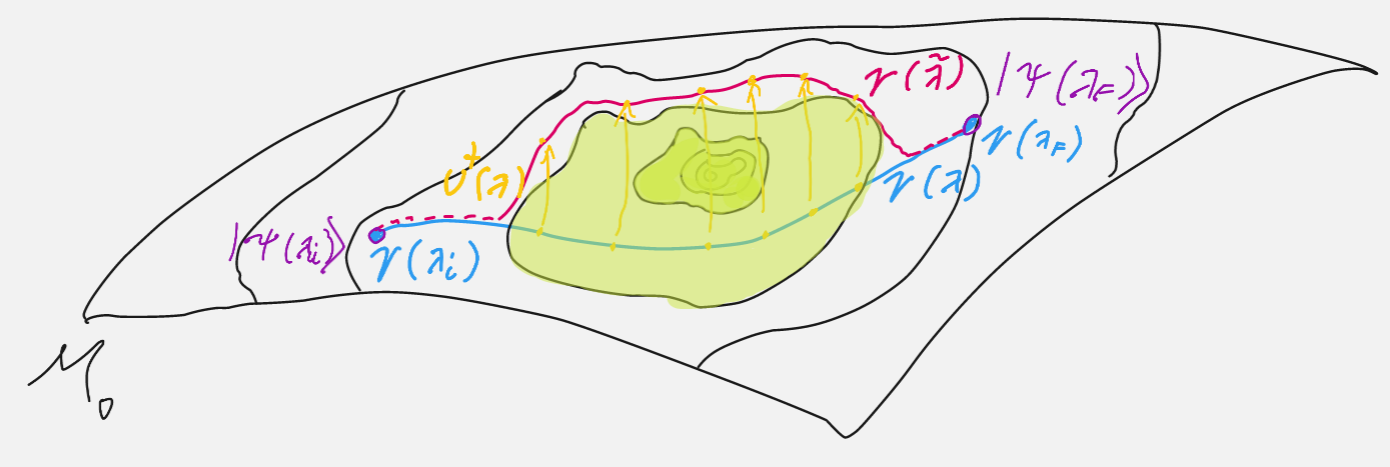
\includegraphics[width=\textwidth]{../img/counterdiabaticPotential.png}
%     \caption{Comparison between transport by Hamiltonian $\HH$ (blue path $\gamma(\lambda)$ and the one with counter-diabatic potential added (pink path $\gamma(\tilde\lambda)$), which has zero fidelity. The nonzero fidelity area for path $\gamma(\lambda)$ is marked green and initial and final states $\ket{\psi(\lambda_i)}$, resp. $\ket{\psi(\lambda_f)}$ are marked purple.}
%     \label{fig:counterdiabaticPotential}
% \end{figure}
This procedure does not directly tell us how to calculate the counter-diabatic potential, only states its existence. For many simple cases the calculation can be done analytically, but most often some approximation methods are needed.


\subsection{Explicit form}
If we now consider the parametrization with time $t\coloneqq t$, $\U$ can be explicitly expressed according to \textcolor{red}{ansatz} in eq. \ref{eq:phasesOnManifold} as
\begin{equation}
    \U(t)=\sum_n \exp\left(\frac{i}{\hbar}E_n(\tau)\d \tau - \int_0^t \braket{s(\tau)|\partial_\tau n(\tau)}\d\tau\right)\ket{s(t)}\bra{s(0)}.
    \label{eq:evolutionUduringTransition}
\end{equation}
Inserting to eq. \ref{eq:schrodingerForU}, we get explicit form of the Hamiltonian, which can be decomposed into the diagonal form of the original Hamiltonian and a counter-diabatic potential
\begin{equation}
    \HH(t)=\sum_n \ket{n}E_n\bra{n}+ i\hbar \sum_n\ket{\partial_\lambda n}\bra{n}-\braket{n|\partial_\lambda n}\ket{n}\bra{n}\eqqcolon \HH_0(t)+\HH_1(t),
\end{equation}
for shortened notation $\ket{n}\equiv \ket{n(t)}$, analogically for bras. Using
\begin{equation}
    \HH_0(t)\ket{n}=E_n\ket{n}\quad \Rightarrow\quad \braket{m|\partial_\lambda n}=\frac{\braket{m|\partial_\lambda\HH_0| n}}{E_n-E_m}
\end{equation}
we have explicit formula
\begin{equation}
    \HH_1(t)= i\hbar \sum_{m\neq n}\frac{\ket{m}\braket{m|\partial_\lambda\HH_0| n}\bra{n}}{E_n-E_m}
    \label{eq:explicitCounterDiabaticPotential}
\end{equation}


\section{Berry phase and curvature}
Let's now consider only the ground state manifold, because it will be used later on. Thought every step can be easily generalized to any state manifold $\M_m$.

On the ground state manifold $\M_0\equiv \cup_\llambda \{\ket{o(\llambda)}\}$, the \emph{Berry connection} is defined as
\begin{equation}
    A_\mu(\llambda)\equiv \braket{o(\llambda)|\AA_\mu|o(\llambda)}=-i\hbar \braket{o(\llambda)|\partial_\mu|o(\llambda)},
    \label{eq:berryConnection}
\end{equation}
which uses the decomposition of $\llambda$ to some basis, thus it empowers us to take derivatives in any direction in the base manifold $\R^n$ and thus the geometric tensor can be written as
\begin{equation}
    \chi_{\mu\nu}(\llambda) = \partial_\mu A_\nu(\llambda)-\partial_\nu A_\mu(\llambda)
\end{equation}
and the \emph{Berry phase}\footnote{
    The reasonability of this definition can be seen, if we assume the ground state of a free particle
        $\braket{\bm{x}|i(\llambda)}=i(\bm{x},\llambda)= |i(\bm{x})|e^{i\phi(\llambda)}$,
    then the Berry connection is
    \begin{equation}
        A_\mu=-\int \d \bm{x}|i(\bm{x},\llambda)|^2\partial_\mu \phi(\llambda) = -\partial_\mu \phi(\llambda)
    \end{equation} 
    and Berry phase
    \begin{equation}
        \phi_B=\oint_\mathcal{C} \partial_\mu \phi \d \lambda^\mu,
    \end{equation}
    which represents total phase accumulated by the wave function. It is really the analogy for Berry phase in classical mechanics, which for example in the case Foucault pendulum on one trip around the Sun makes $\phi_B=2\pi$
}
as the integral of a connection along some closed curve $\mathcal{C}$
\begin{equation}
    \phi_B\equiv-\oint_\mathcal{C} A_\mu(\llambda)\d \lambda^\mu=\int_\mathcal{S} \chi_{\mu\nu}(\llambda)\d \lambda^\mu \wedge \d\lambda^\nu,
\end{equation}
where we used the Stokes theorem for some area $\mathcal{S}$ with boundary $\partial\mathcal{S}=\mathcal{C}$.




\section{\textcolor{blue}{Approximations of adiabatic potentials}}
Adiabatic potentials can be calculated from the principal of minimal action, which leads to variational method.

If the difference between eigenstates of $\HH$ is small, or generalized force between some states is zero, the computation of the adiabatic potential is numerically unstable. The knowledge of exact adiabatic potential would allow to maintain the system in the ground state thus not exciting it, as the Eigenstate thermalization hypotheses states.

\begin{hypot}[Eigenstate thermalization hypotheses]
  For the difference between eigenstates of $\HH$ and extensive thermodynamic entropy $S$, it holds that
    \begin{equation}
    E_n-E_m\propto \exp\left(\frac{S}{2}\right).
  \end{equation}
  If the states are close, better approximation would be $E_n-E_m\propto \exp(S)$. For matrix elements it holds, that they vanish exponentially with the characteristic scale of the system $a$, i.e.
  \begin{equation}
    \bra{m}\AA_\lambda\ket{n} = i\hbar\frac{\braket{m|\partial_\lambda \HH|n}}{E_m-E_n} \propto \exp(-a).
    \label{eq:thermalizationMatrixElements}
\end{equation}
\end{hypot}
Fortunately in the limit "number of particles" $\rightarrow \infty$ the expression in eq. \ref{eq:thermalizationMatrixElements} converges.



\subsection{Variational methods}
In the case of simple systems, the adiabatic potentials can be found analytically, but for more complicated Hamiltonians we will be forced to use approximations, or some perturbational and variational methods.
\chapter{\textcolor{blue}{Geodesics}}
Of special importance in theory of the ground state manifold are geodesics. It is not yet clear what role they have in general, but in some special cases its well known, see \cite{polkovnikov}. The holy grail of this theory would be to find path with the lowest excitation amplitude, which is not an easy task.

Let's have a geodesic $\mathcal{G}(t)$ and some curve $\gamma(t)$ on the ground stat manifold, spanning between points $P_i$ and $P_f$ during some time $t_f$, meaning
 $$\mathcal{G}(0)=\gamma(0)=P_i\in\mathcal{M}_0,\qquad \mathcal{G}(t_f)=\gamma(t_f)=P_f\in\mathcal{M}_0.$$

Excitation amplitude during infinitesimal quench is $\d s$, therefore $\sum_i \Delta s_i$ summed along path $\gamma(t)$ is the amplitude of transport along that path. This can be more rigorously expressed by functional
\begin{equation}
    s_\gamma=\int_{\gamma(t)}\d s=\int_{0}^{t_f}\sqrt{g_{\mu\nu}\dot\lambda^\mu\dot\lambda^\nu}\d t
\end{equation}
This is the entity, which is minimal if $\gamma$ is a geodesic. Before moving on, lets quickly review the proof of this statement.

\begin{proof}[Geodesics minimize the distance on manifold]
    Functional of distance is
    \begin{equation}
        s=\int\mathcal{L}(t,\lambda^\mu,\dot\lambda^\mu)\d t
    \end{equation}
    for 
    \begin{equation}
        \mathcal{L}=\sqrt{g_{\mu\nu}\dot\lambda^\mu\dot\lambda^\nu}.
    \end{equation}
    Using Euler-Lagrange equations 
    \begin{equation}
        \der{\mathcal{L}}{\lambda^\mu}-\der{}{t}\der{\mathcal{L}}{\dot\lambda^\mu}=0,
    \end{equation}
    we get for $g_{\mu\nu}=g_{\mu\nu}(\lambda^\mu)$ second order differential equation
    \begin{equation}
        \ddot\lambda^\mu+\Gamma^\mu_{\;\;\alpha\beta}\dot\lambda^\alpha\dot\lambda^\beta=0\qquad \Gamma^\mu_{\;\;\alpha\beta}=\frac{1}{2}g^{\mu\kappa}\left(g_{\kappa\alpha,\beta}+g_{\kappa\beta,\alpha}-g_{\beta\alpha,\kappa}\right),
        \label{eq:geodesicEquaiton}
    \end{equation}
    which is the Geodesic equation.
\end{proof}

Excitation probability along the path $\gamma$ can be formally written as $F=\sum_i\Delta s_i^2$, which cannot be simply calculated as $s^2$. Because $\Delta s_i>0$, we have
\begin{equation}
    \begin{split}
        \sum_i \Delta s_i^2& <(\sum_i\Delta s_i)^2\\
        F&<s^2.
    \end{split}
\end{equation}

This doesn't necessarily mean, that fidelity along geodesic will be minimal ($F(\mathcal{G})<F(\gamma)$), because we didn't rule out the scenario 
$$F(\gamma)<F(\mathcal{G})<s_\mathcal{G}^2<s_\gamma^2.$$

This means, that the geodesic equation cannot be used for fidelity minimization and some new insight is needed. The functional, which needs to be minimized is
\begin{equation}
    F=\int\int g_{\mu\nu}\d\lambda^\mu\d\lambda^\nu = \int_{t_i}^{t_f}\underbrace{\int_{t_i}^\tau g_{\mu\nu}\der{\lambda^\mu}{t}\der{\lambda^\nu}{t} \d t}_{\mathcal{L}(\lambda^\mu,\dot\lambda^\mu,\tau)}\d \tau .
\end{equation}
Using Euler-Lagrange equations, again for time independent $g_{\mu\nu}=g_{\mu\nu}(\lambda^\mu)$, leads to
\begin{equation}
    \int_{t_i}^{t_f}\left[g_{\mu\nu,\kappa}\dot\lambda^\mu\dot\lambda^\nu - \der{}{t}\left[g_{\mu\nu}\left(\delta^\mu_\kappa\dot\lambda^\mu+\dot\lambda^\mu\delta^\nu_\kappa\right)\right]\right]\d t=0
\end{equation}
which needs to be zero for integration over any subset $(t_i,t_f)$ leading to zero condition for the integrand itself, which leads to geodesic equation \ref{eq:geodesicEquaiton}, as in the case of distance on manifold.



\textcolor{blue}{Polkovnikov for some special case: They play a role of "maximum fidelity at any time" transport, meaning at any given time $t$ the fidelity on corresponding point on geodesics will be less than of $\gamma$
$$F(\mathcal{G}(t))<F(\gamma(t)).$$ }



\chapter*{Conclusion}
\addcontentsline{toc}{chapter}{Conclusion}
This thesis presents the theory of quantum state driving theory of finite Hamiltonian systems. The well known claims were reformulated into more rigorous theorems and definitions style of writing. This mathematical approach has potential to reduce the barrier for any mathematically based scientist without training in quantum mechanics when trying to approach this theory. The playground in the form of fiber space was constructed, and the geometry of energy states reformulated on it. Some theorems were proposed based on previous knowledge from the area of physics concerning quantum state driving, and clear definitions of generally used terms were presented.

The correspondence to a damped harmonic oscillator in the fidelity behavior was shown on a simple two-level system. In the case of geodesic driving, the fidelity oscillates with constant frequency and periodically becomes one. For linear driving, the fidelity has essentially two regimes — fast transport regime, described by the semiclassical Landau-Zener formula, and close adiabatic regime, described by APT. In both models, the fidelity is excited when the difference between energy levels gets small. These excitations lead to damped oscillations.

In the LMG model, the ground state manifold is analyzed. The Riemannian manifold characteristics were calculated along with their implications. These are ground state manifold geodesics and coordinates of diabolic points in parametric space, dependent on the Hamiltonian dimension. In three dimensions, this was done analytically, proving the existence of diabolic points. For higher dimensions, numerical methods were used. The transport using quenches was numerically demonstrated, showing the transformation to adiabatic transport by shortening the quenches.

Many questions still lay unsolved, and some were newly opened. For example: "What are the possibilities for quantum quench transport?". "What is the correspondence of energy variance and driving fidelity?". Further on, from the LMG model, the proposed analytical formula for diabolic points coordinates remains to be proven analytically, along with the number of these points.

This thesis provides a significant amount of numerical analysis on two quantum models, which will hopefully serve for future discoveries in this area of physics. The state manifold analyses might lead the search for better fidelity protocols, or maybe the geodesics will be found to be somewhat "most stable protocols" for counter-diabatic driving. Either way, the possibilities are yet open and not known.

%%% Bibliography
%%% Bibliography (literature used as a source)
%%%
%%% We employ bibTeX to construct the bibliography. It processes
%%% citations in the text (e.g., the \cite{...} macro) and looks up
%%% relevant entries in the bibliography.bib file.
%%%
%%% The \bibliographystyle command selects, which style will be used
%%% for references from the text. The argument in curly brackets is
%%% the name of the corresponding style file (*.bst). Both styles
%%% mentioned in this template are included in LaTeX distributions.
\bibliographystyle{unsrtnat}
% \bibliographystyle{plainnat}    %% Author (year)
% \bibliographystyle{unsrt}     %% [number]

\renewcommand{\bibname}{Bibliography}

%%% Generate the bibliography. Beware that if you cited no works,
%%% the empty list will be omitted completely.

\bibliography{bibliography}

%%% If case you prefer to write the bibliography manually (without bibTeX),
%%% you can use the following. Please follow the ISO 690 standard and
%%% citation conventions of your field of research.

% \begin{thebibliography}{99}
%
% \bibitem{lamport94}
%   {\sc Lamport,} Leslie.
%   \emph{\LaTeX: A Document Preparation System}.
%   2nd edition.
%   Massachusetts: Addison Wesley, 1994.
%   ISBN 0-201-52983-1.
%
% \end{thebibliography}


%%% Figures used in the thesis (consider if this is needed)
\listoffigures

%%% Tables used in the thesis (consider if this is needed)
%%% In mathematical theses, it could be better to move the list of tables to the beginning of the thesis.
%\listoftables

%%% Abbreviations used in the thesis, if any, including their explanation
%%% In mathematical theses, it could be better to move the list of abbreviations to the beginning of the thesis.
%\chapwithtoc{List of Abbreviations}

%%% Attachments to the master thesis, if any. Each attachment must be
%%% referred to at least once from the text of the thesis. Attachments
%%% are numbered.
%%%
%%% The printed version should preferably contain attachments, which can be
%%% read (additional tables and charts, supplementary text, examples of
%%% program output, etc.). The electronic version is more suited for attachments
%%% which will likely be used in an electronic form rather than read (program
%%% source code, data files, interactive charts, etc.). Electronic attachments
%%% should be uploaded to SIS and optionally also included in the thesis on a~CD/DVD.
%%% Allowed file formats are specified in provision of the rector no. 72/2017.
\appendix
\chapter{Attachments}

\section{First Attachment}

\openright
\end{document}
